\documentclass[a4paper,12pt]{article}
\usepackage[12pt]{extsizes}
\usepackage[T2A]{fontenc}
\usepackage[utf8]{inputenc}
\usepackage[english, russian]{babel}
\usepackage[left=3cm,right=1.5cm,top=2cm,bottom=2cm]{geometry}
\usepackage{hyperref}
\usepackage{amssymb,amsmath,amsthm}
\usepackage{cleveref}
\usepackage{caption}
\usepackage{mathtools}
\usepackage{multirow}

%\usepackage{subfig}  % или \usepackage{subcaption}
\usepackage{graphicx} % Required for inserting images
\usepackage{ulem}
\usepackage{amsmath}
\usepackage{geometry}
\geometry{top=2.5cm, bottom=2.5cm, left=2.5cm, right=2.5cm}
\usepackage{hyperref}
\usepackage{array}
\usepackage{booktabs}  % Для более красивых таблиц (по желанию)
\usepackage{tabularx}
\usepackage{enumitem}
%\usepackage{titlesec}
\usepackage{appendix}
\usepackage{float}    % Для принудительной вставки картинок в определенное место (чтобы они не "плавали") [H]
\usepackage{subcaption}   % для окружений subfigure
\usepackage{indentfirst}
\usepackage[nottoc,numbib]{tocbibind} % Пакет tocbibind добавляет в оглавление пункты, которые обычно туда не попадают: библиографию, список иллюстраций, список таблиц и т. д.


\sloppy
\emergencystretch=1em

\begin{document}

% --------------------- Титульник ВКР СПбГУ -----------------------------
% Автор: Тоскин Николай, itonik@me.com
% Если заметили ошибку, напишите на email
% Если хотите добавить изменение самостоятельно:
% https://github.com/itonik/spbu_diploma/
% Использованы материалы:
% habr.com/ru/post/144648/
% cpsconf.ru
% Документы ниже могут уже быть неактуальны, тем не менее за годы ничего
% нового не появилось
% Текст:
% http://edu.spbu.ru/images/data/normativ_acts/local/20181030_10432_1.pdf
% Титульный лист:
% http://edu.spbu.ru/images/data/normativ_acts/local/20180703_6616_1.pdf
% -----------------------------------------------------------------------

% Титульный лист диплома СПбГУ
% Временное удаление foot на titlepage
\newgeometry{left=30mm, top=20mm, right=15mm, bottom=20mm, nohead, nofoot}
\begin{titlepage}
\begin{center}

\textbf{Санкт--Петербургский}
\textbf{государственный университет}

\vspace{35mm}

\textbf{\textit{\large Соловьев Дмитрий Николаевич}} \\[8mm]
% Название
\textbf{\large Выпускная квалификационная работа}\\[3mm]
\textbf{\textit{\large Система домашней автоматизации с использованием децентрализованного подхода в хранении и обработке данных.}}

\vspace{20mm}
Уровень образования: бакалавриат\\
Направление 02.03.02  «Фундаментальная информатика и информационные технологии»\\
Основная образовательная программа CB.5190.2021
«Большие данные и распределенная цифровая платформа»\\[25mm]
%Профиль «Исследование и проектирование систем управления\\ и обработки сигналов»\\[25mm]


% Научный руководитель, рецензент
\begin{flushright}
\begin{minipage}[t]{0.65\textwidth}
{Научный руководитель:} \\
доцент, кафедра компьютерного моделирования и \\многопроцессорных систем,\\к.ф.-м.н., PhD\\Корхов Владимир Владиславович

\vspace{10mm}

{Рецензент:} \\
доцент, кафедра компьютерного моделирования и \\многопроцессорных систем,\\к.т.н.\\Дик Геннадий Давидович
\end{minipage}
\end{flushright}

\vfill 

{Санкт-Петербург}
\par{\the\year{} г.}
\end{center}
\end{titlepage}
% Возвращаем настройки geometry обратно (то, что объявлено в преамбуле)
\restoregeometry
% Добавляем 1 к счетчику страниц ПОСЛЕ titlepage, чтобы исключить 
% влияние titlepage environment
\addtocounter{page}{1}

%% --------------------- Титульник ВКР СПбГУ -----------------------------
% Автор: Тоскин Николай, itonik@me.com
% Если заметили ошибку, напишите на email
% Если хотите добавить изменение самостоятельно:
% https://github.com/itonik/spbu_diploma/
% Использованы материалы:
% habr.com/ru/post/144648/
% cpsconf.ru
% Документы ниже могут уже быть неактуальны, тем не менее за годы ничего
% нового не появилось
% Текст:
% http://edu.spbu.ru/images/data/normativ_acts/local/20181030_10432_1.pdf
% Титульный лист:
% http://edu.spbu.ru/images/data/normativ_acts/local/20180703_6616_1.pdf
% -----------------------------------------------------------------------

% Титульный лист диплома СПбГУ
% Временное удаление foot на titlepage
\newgeometry{left=30mm, top=20mm, right=15mm, bottom=20mm, nohead, nofoot}
\begin{titlepage}
\begin{center}

\textbf{Санкт--Петербургский}
\textbf{государственный университет}

\vspace{35mm}

\textbf{\textit{\large Соловьев Дмитрий Николаевич}} \\[8mm]
% Название
\textbf{\large Отчет по учебной практике }\\[3mm]
\textbf{\textit{\large Система домашней автоматизации с использованием децентрализованного подхода в хранении и обработке данных.}}

\vspace{20mm}
Уровень образования: бакалавриат\\
Направление 02.03.02  «Фундаментальная информатика и информационные технологии»\\
Основная образовательная программа CB.5190.2021
«Большие данные и распределенная цифровая платформа»\\[25mm]
%Профиль «Исследование и проектирование систем управления\\ и обработки сигналов»\\[25mm]


% Научный руководитель, рецензент
\begin{flushright}
\begin{minipage}[t]{0.65\textwidth}
{Научный руководитель:} \\
доцент, кафедра компьютерного моделирования и \\многопроцессорных систем,\\ кандидат физико-математических наук, PhD\\Корхов Владимир Владиславович

\vspace{10mm}

{Руководитель практики:} \\
профессор, кафедра фундаментальной информатики и\\ распределенных систем,\\ доктор физико-математических наук, \\Богданов Александр Владимирович
\end{minipage}
\end{flushright}

\vfill 

{Санкт-Петербург}
\par{\the\year{} г.}
\end{center}
\end{titlepage}
% Возвращаем настройки geometry обратно (то, что объявлено в преамбуле)
\restoregeometry
% Добавляем 1 к счетчику страниц ПОСЛЕ titlepage, чтобы исключить 
% влияние titlepage environment
\addtocounter{page}{1}




\section*{Аннотация}

С увеличением количества устройств интернет вещей (ИВ) в системах домашней автоматизации (СДА) остро встает вопрос топологий сетей, в которых находятся эти устройства, а также способах хранения и передачи данных между устройствами. Многим системам, использующим централизованный подход в хранении и обработке информации, свойственна существенная потеря функциональности при выходе из строя центрального узла. В ходе исследования были изучены принципы, методологии и архитектуры, применимые к программно-аппаратным комплексам для построения СДА и позволяющие повысить уровень безопасности данных, отказоустойчивость и увеличить скорость передачи информации в рамках системы за счет использования распределенного подхода к хранению и обработке информации, разработан прототип распределенной СДА. Результаты проведенного исследования и предложенная в нем архитектурная модель могут быть использованы не только в системах умных домов, но и в умных городах и на предприятиях.

\section*{Abstract}

With the increasing number of Internet of Things (IoT) devices in home automation systems (HAS), the topologies of the networks that house these devices, as well as how data is stored and transferred between devices, are becoming an issue. Many systems that use a centralized approach in storing and processing information are characterized by a significant loss of functionality when a central node fails. In the course of the research the principles, methodologies and architectures applicable to hardware-software complexes for the construction of ADS were studied, which allow to increase the level of data security, fault tolerance and increase the speed of information transfer within the system due to the use of distributed approach to information storage and processing, and a prototype of distributed ADS was developed. The results of the conducted research and the architectural model proposed in it can be used not only in smart home systems, but also in smart cities and enterprises.

\newpage

\tableofcontents

\newpage


%%%%%%%%%%%%%%%%%%%%%%%%%%%%%%%%%%%%%%%%%%%%%%%%%%%%%%%%%%%%%%%%%%%%%%%%%%%%%%%%%%%%%%%%%%%%%%%%%%%%%%%%%%%%%%%%%%%%%%%%%%%%%%%%%%%%%%%%%%%%%%%%%%%%%%%%%%%%%%%%%%%%%%%%%%%%%
%%%%%%%%%%%%%%%%%%%%%%%%%%%%%%%%%%%%%%%%%%%%%%%%%%%%%%%%%%%%%%%%%%%%%%%%%%%%%%%%%%%%%%%%%%%%%%%%%%%%%%%%%%%%%%%%%%%%%%%%%%%%%%%%%%%%%%%%%%%%%%%%%%%%%%%%%%%%%%%%%%%%%%%%%%%%%
%%%%%%%%%%%%%%%%%%%%%%%%%%%%%%%%%%%%%%%%%%%%%%%%%%%%%%%%%%%%%%%%%%%%%%%%%%%%%%%%%%%%%%%%%%%%%%%%%%%%%%%%%%%%%%%%%%%%%%%%%%%%%%%%%%%%%%%%%%%%%%%%%%%%%%%%%%%%%%%%%%%%%%%%%%%%%
%                                                                                                                                                                           %
%                                                            ВВЕДЕНИЕ. Актуальность, постановка задачи и т.д                                                                %
%                                                                                                                                                                           %
%%%%%%%%%%%%%%%%%%%%%%%%%%%%%%%%%%%%%%%%%%%%%%%%%%%%%%%%%%%%%%%%%%%%%%%%%%%%%%%%%%%%%%%%%%%%%%%%%%%%%%%%%%%%%%%%%%%%%%%%%%%%%%%%%%%%%%%%%%%%%%%%%%%%%%%%%%%%%%%%%%%%%%%%%%%%%
%%%%%%%%%%%%%%%%%%%%%%%%%%%%%%%%%%%%%%%%%%%%%%%%%%%%%%%%%%%%%%%%%%%%%%%%%%%%%%%%%%%%%%%%%%%%%%%%%%%%%%%%%%%%%%%%%%%%%%%%%%%%%%%%%%%%%%%%%%%%%%%%%%%%%%%%%%%%%%%%%%%%%%%%%%%%%
%%%%%%%%%%%%%%%%%%%%%%%%%%%%%%%%%%%%%%%%%%%%%%%%%%%%%%%%%%%%%%%%%%%%%%%%%%%%%%%%%%%%%%%%%%%%%%%%%%%%%%%%%%%%%%%%%%%%%%%%%%%%%%%%%%%%%%%%%%%%%%%%%%%%%%%%%%%%%%%%%%%%%%%%%%%%%


\section{Введение}

\subsection{Актуальность темы}

Актуальность и практический аспект анализа систем и выбора оптимальной для построения системы домашней автоматизации:

\begin{enumerate}
    \item	Количество устройств с возможностью интеграции в систему умного дома среди потребителей быстро возрастает год к году. Особенности построения актуальных систем накладывает ограничения на масштабируемость системы, ее надежность и безопасность.
    \item	В системах домашней автоматизации с появлением новых типов устройств и попытки их интеграции возникают проблемы, связанные со скоростью реакции на события и с отсутствием приоритезации сообщений.
\end{enumerate}

\subsection{Объект исследования}


Объектом научно-исследовательской работы являются системы домашней автоматизации, системы хранения, передачи и обработки информации.


\subsection{Предмет исследования}



Предметом научно-исследовательской работы является оптимизация обработки и передачи данных между устройствами ИВ в системе домашней автоматизации.

\subsection{Постановка задачи}


В рамках данной работы ставится цель провести комплексное исследование существующих СДА на рынке, проанализировать применяемые в них протоколы и выявить основные недостатки. На основании этого выбрать оптимальный протокол и разработать прототип системы, отвечающий сформулированным требованиям и решающий обозначенный список проблем.

Для достижения этой цели были сформулированы начальные условия (требования):

\begin{enumerate}
    \item Сеть устройств в пределах одной зоны должна строиться по одноуровневому принципу, без централизованных узлов управления.
    \item Взаимодействие устройств внутри зоны осуществляется напрямую, без посредников (ЦУД).
    \item Для связи устройств из разных зон используются шлюзы-ретрансляторы, объединённые в единую распределённую сеть.
\end{enumerate}

\paragraph{Практическая значимость предлагаемого подхода:}
\begin{itemize}
    \item Уменьшение задержек, расширение сфер применения: в предлагаемой системе уменьшается количество узлов между устройством-инициатором и устройством-актуатором (при нахождении в одной сети - до нуля), за счет чего увеличивается скорость выполнения команд и повышается общая отзывчивость системы, что расширяет сферы применения устройств ИВ для построения СДА, ранее нефункциональных ввиду относительно больших задержек.
    \item Повышение комфорта использования: данные о состоянии устройств, как и статистика, собираемая устройствами, хранится и обрабатывается на самих устройствах, что позволяет обеспечить короткое время восстановления работы после внештатных ситуаций (например, отключения питания) без длительной синхронизации.
    \item Упрощение настройки системы: благодаря использованию планировщика, автоматически распределяющего сценарии по устройствам, нет необходимости в ручной конфигурации каждого узла.
    \item Повышение отказоустойчивости: отказ сценария в одной локации возможен лишь при неисправности одного из двух устройств (инициатора и актуатора) и не зависит от иных устройств в сети. Объединение локаций, а также дистанционный мониторинг и управление системой осуществляется посредством распределенной системы шлюзов-ретрансляторов, что избавляет от единой точки отказа системы (точки входа).
    \item Повышение безопасности: распределенный подход для хранения сценариев и управления устройствами минимизирует получение злоумышленниками доступа ко всем устройствам. Система шлюзов-ретрансляторов, использующих VPN-соединение избавляет от единой точки отказа системы (точки входа).

\end{itemize}



%%%%%%%%%%%%%%%%%%%%%%%%%%%%%%%%%%%%%%%%%%%%%%%%%%%%%%%%%%%%%%%%%%%%%%%%%%%%%%%%%%%%%%%%%%%%%%%%%%%%%%%%%%%%%%%%%%%%%%%%%%%%%%%%%%%%%%%%%%%%%%%%%%%%%%%%%%%%%%%%%%%%%%%%%%%%%
%%%%%%%%%%%%%%%%%%%%%%%%%%%%%%%%%%%%%%%%%%%%%%%%%%%%%%%%%%%%%%%%%%%%%%%%%%%%%%%%%%%%%%%%%%%%%%%%%%%%%%%%%%%%%%%%%%%%%%%%%%%%%%%%%%%%%%%%%%%%%%%%%%%%%%%%%%%%%%%%%%%%%%%%%%%%%
%%%%%%%%%%%%%%%%%%%%%%%%%%%%%%%%%%%%%%%%%%%%%%%%%%%%%%%%%%%%%%%%%%%%%%%%%%%%%%%%%%%%%%%%%%%%%%%%%%%%%%%%%%%%%%%%%%%%%%%%%%%%%%%%%%%%%%%%%%%%%%%%%%%%%%%%%%%%%%%%%%%%%%%%%%%%%
%                                                                                                                                                                           %
%                                                       ГЛАВА I. Топологии сетей и протоколы беспроводных сетей                                                             %
%                                                                                                                                                                           %
%%%%%%%%%%%%%%%%%%%%%%%%%%%%%%%%%%%%%%%%%%%%%%%%%%%%%%%%%%%%%%%%%%%%%%%%%%%%%%%%%%%%%%%%%%%%%%%%%%%%%%%%%%%%%%%%%%%%%%%%%%%%%%%%%%%%%%%%%%%%%%%%%%%%%%%%%%%%%%%%%%%%%%%%%%%%%
%%%%%%%%%%%%%%%%%%%%%%%%%%%%%%%%%%%%%%%%%%%%%%%%%%%%%%%%%%%%%%%%%%%%%%%%%%%%%%%%%%%%%%%%%%%%%%%%%%%%%%%%%%%%%%%%%%%%%%%%%%%%%%%%%%%%%%%%%%%%%%%%%%%%%%%%%%%%%%%%%%%%%%%%%%%%%
%%%%%%%%%%%%%%%%%%%%%%%%%%%%%%%%%%%%%%%%%%%%%%%%%%%%%%%%%%%%%%%%%%%%%%%%%%%%%%%%%%%%%%%%%%%%%%%%%%%%%%%%%%%%%%%%%%%%%%%%%%%%%%%%%%%%%%%%%%%%%%%%%%%%%%%%%%%%%%%%%%%%%%%%%%%%%

\newpage

\section{Глава 1. Топологии сетей и протоколы беспроводных сетей}

\subsection{Топологии беспроводных сетей}
Все перечисленные беспроводные сети работают в одном или нескольких вариантах
топологии. На рис.~\ref{fig:topologies} приведены топологии беспроводных сетей различных конфигураций.

\begin{figure}[h]
    \centering
    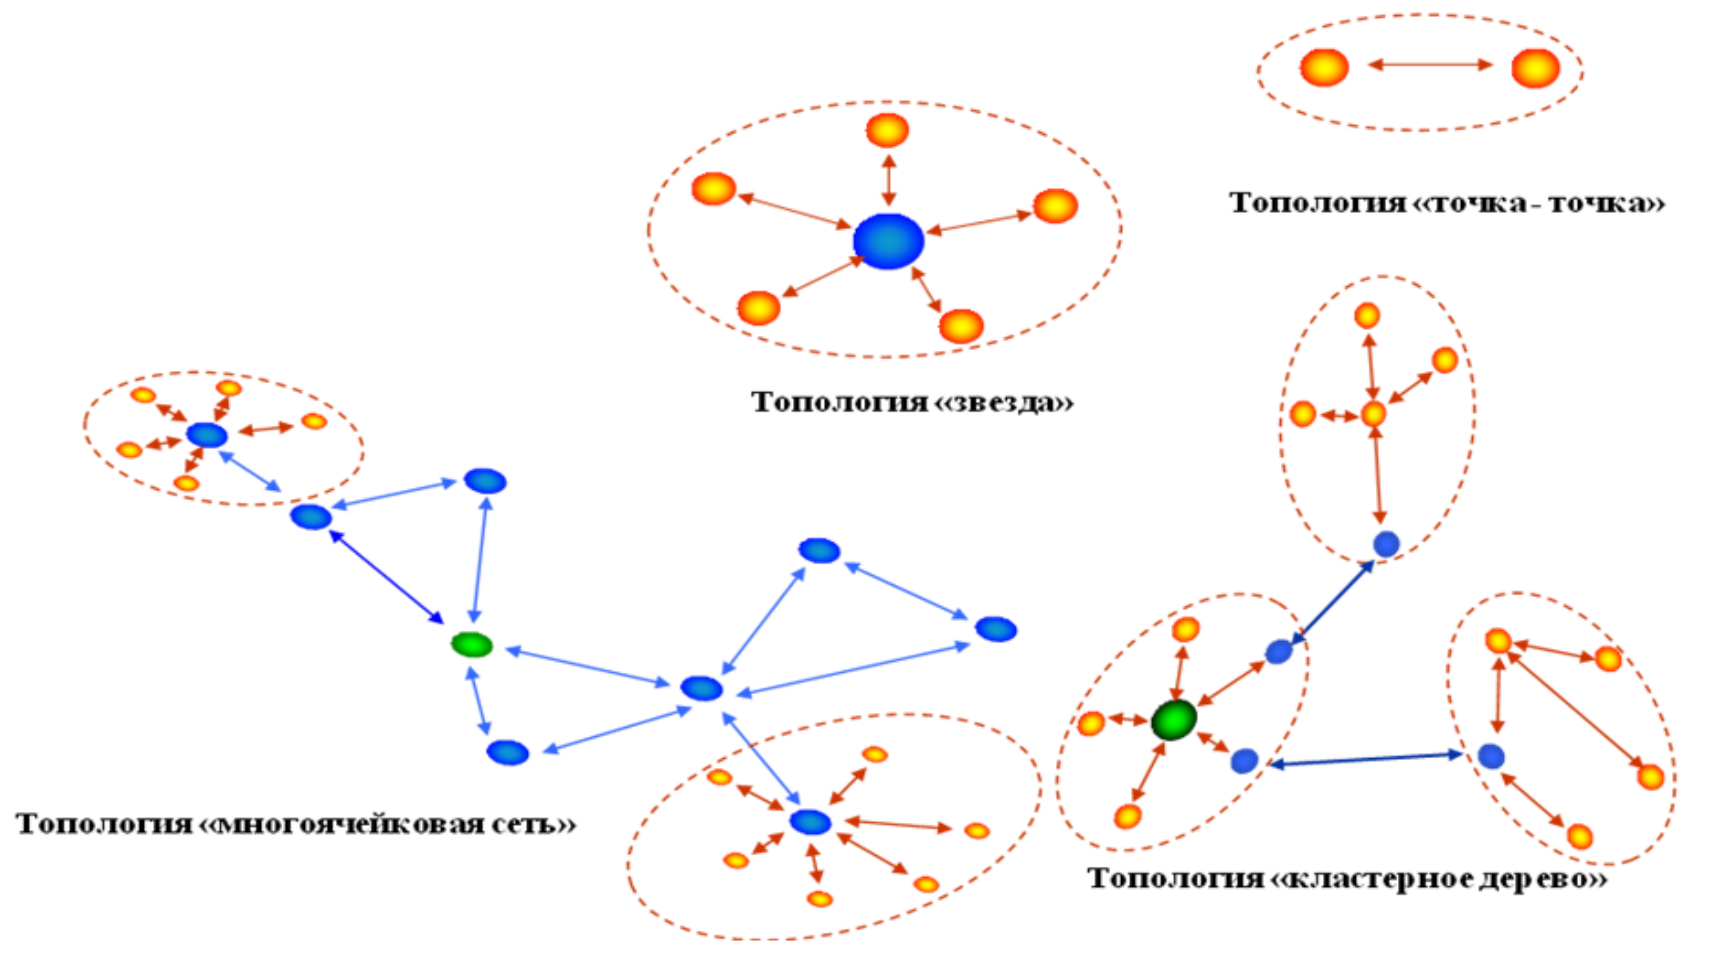
\includegraphics[width=0.8\textwidth]{images/Fig06.png}
    \caption{Топологии беспроводных сетей \cite{wirelessNetProtocols} }
    \label{fig:topologies}
\end{figure}



\subsubsection{Топология точка-точка}
Самый простой вариант организации сети из двух устройств. Как правило, узлы этой сети являются равноправными, то есть сеть одноранговая.
Эта топология характерна для Bluetooth, ANT, RFID, RuBee, PDC, WI-FI, Insteon, UWB, ZigBee и прочих.

\subsubsection{Топология «Звезда»}
Эта топология служит основой организации всех современных сетей связи и вычислительных сетей. Данную топологию используют протоколы WI-FI, Insteon, ZigBee, UWB, IDEN, CDMAOne, WIMAX, GSM, GPRS, UTMS.

\subsubsection{Ячеистая топология}
Ячеистая топология — базовая полносвязная топология компьютерных сетей и сетей связи, в которой каждая рабочая станция сети соединяется со всеми другими рабочими станциями этой же сети. Характеризуется высокой отказоустойчивостью, сложностью настройки и избыточным расходом кабеля в проводных сетях. Каждый узел имеет несколько возможных путей соединения с другими узлами, за счет этого такая топология очень устойчива. Так как исчезновение одного из каналов не приводит к потере соединения между двумя компьютерами. Эта топология допускает соединение большого количества узлов и характерна, как правило, для крупных сетей, она строится из полносвязной путем удаления некоторых возможных связей.
Топология применима для сетей с использованием протоколов UWB, WI-FI, Insteon, ZigBee, UWB, IDEN, CDMAOne, WIMAX, GSM, GPRS, UTMS.

\subsubsection{Топология «кластерное дерево»}
Топология «Кластерное дерево» образуется в основном в виде комбинаций вышеназванных топологий вычислительных сетей. Основание дерева вычислительной сети располагается в точке (корень), в которой собираются коммуникационные линии информации (ветви дерева).
Вычислительные сети с древовидной структурой строятся там, где невозможно непосредственное применение базовых сетевых структур в чистом виде.


\subsection{Протоколы беспроводных сетей}
В данный момент большинство производителей ИВ используют централизованный подход для построения СДА \cite{Rus_alternative}. В качестве центра умного дома (ЦУД) выступает устройство (хаб), объединяющее конечные устройства в единую сеть. Сценарии взаимодействия устройств могут быть локальными (сценарии хранятся в ЦУД) или облачными. Вариант с локальным расположением сценариев более предпочтительный, так как повышается отзывчивость системы и ее отказоустойчивость. Отдельную сложность представляет объединение устройств из разных экосистем: различные комбинации связей <<устройство>>, <<ЦУД>>, <<облако>>.
\begin{figure}[h]
    \centering
    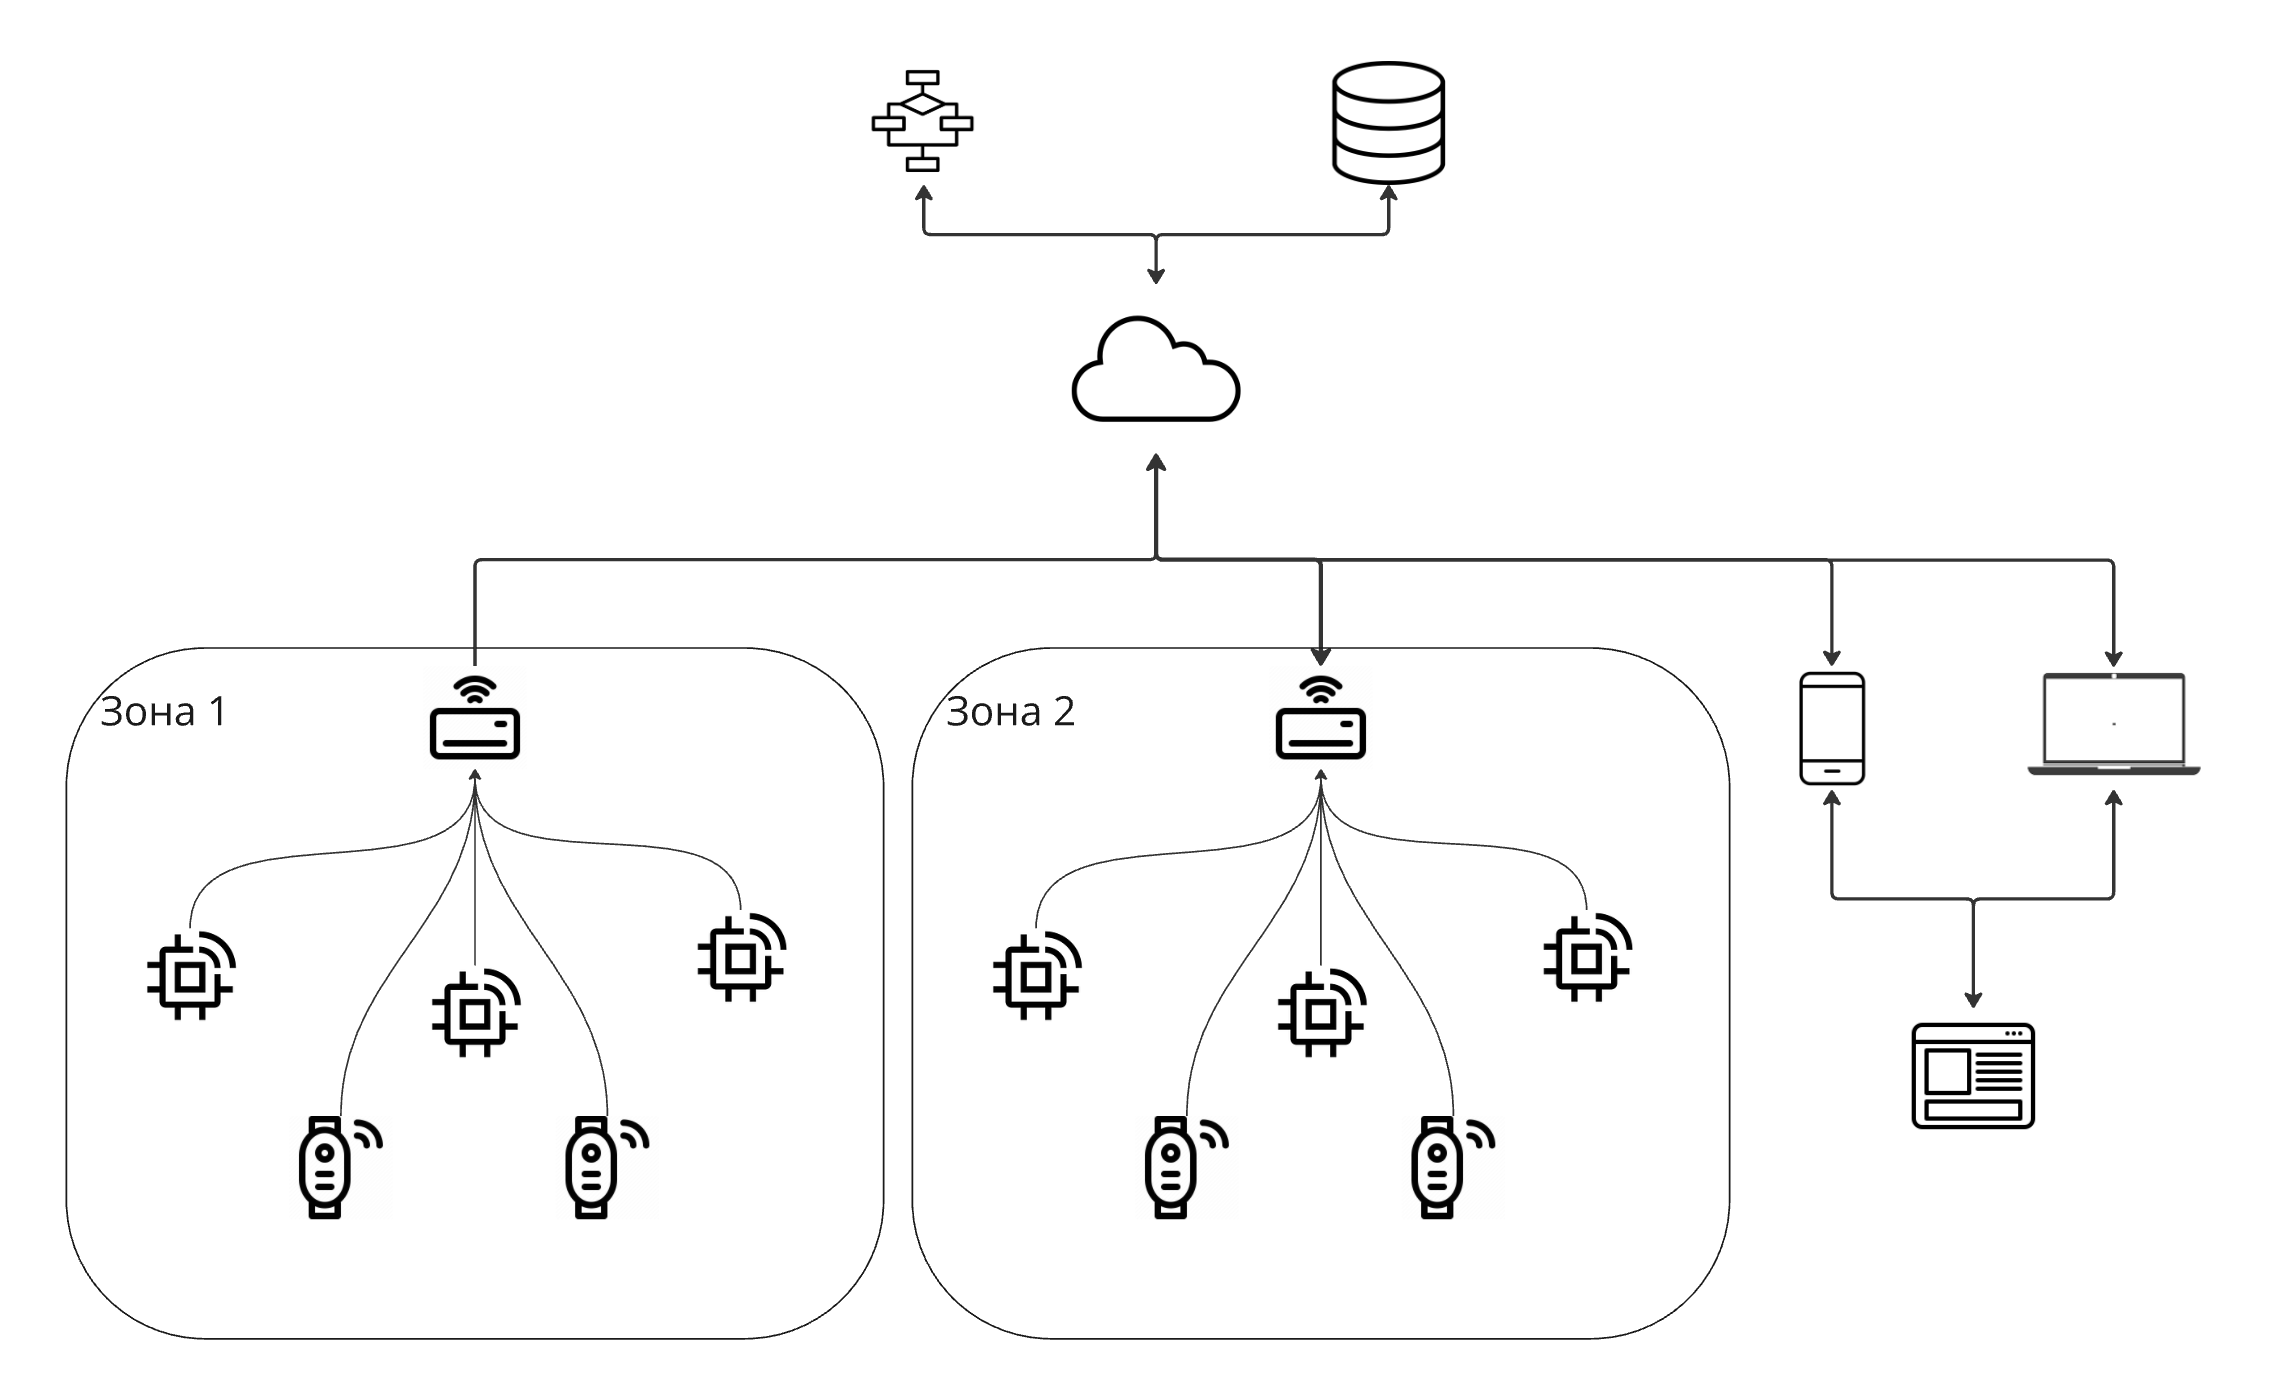
\includegraphics[width=0.8\textwidth]{images/CommertialAlternativeDesign.png}
    \caption{Пример СДА с облачной обработкой событий}
    \label{fig:cloud_event_processing}
\end{figure}

Большинство имеющихся на данный момент решений опираются на топологию <<дерево>>, где в качестве корня рассматривается ЦУД или облако, что проиллюстрированно на рис. \ref{fig:cloud_event_processing}. При этом структура может подразумевать наличие единственных ветвей из корня, например <<облако-ЦУД-устройства>> \cite{smart_home_review}. Тенденции 2023-2024 г. по переносу обработки событий в ЦУД, который ранее использовался лишь для маршрутизации сообщений от устройств к облаку, позволили увеличить надежность и уменьшить задержки в системе, но не исключили имеющиеся проблемы полностью.

Стоит различать аппаратные ограничения, не позволяющие изменить топологию системы, связанные с особенностью работы протокола, например, топологию Bluetooth, позволяющую организовывать только связи типа точка-точка или точка - множество устройств, и архитектуру системы УД, подразумевающую централизованное выполнение сценария в ЦУД либо облаке.


%%%%%%%%%%%%%%%%%%%%%%%%%%%%%%%%%%%%%%%%%%%%%%%%%%%%%%%%%%%%%%%%%%%%%%%%%%%%%%%%%%%%%%%%%%%%%%%%%%%%%%%%%%%%%%%%%%%%%%%%%%%%%%%%%%%%%%%%%%%%%%%%%%%%%%%%%%%%%%%%%%%%%%%%%%%%%
%                                                                                                                                                                           %
%                                                                            Wi-Fi и Wi-Fi HaLow                                                                            %
%                                                                                                                                                                           %
%%%%%%%%%%%%%%%%%%%%%%%%%%%%%%%%%%%%%%%%%%%%%%%%%%%%%%%%%%%%%%%%%%%%%%%%%%%%%%%%%%%%%%%%%%%%%%%%%%%%%%%%%%%%%%%%%%%%%%%%%%%%%%%%%%%%%%%%%%%%%%%%%%%%%%%%%%%%%%%%%%%%%%%%%%%%%
\subsubsection{Wi-Fi и Wi-Fi HaLow}

Протокол Wi-Fi относится к семейству стандартов IEEE 802.11, реализующих беспроводную передачу данных в различных частотных диапазонах:
\begin{itemize}
    \item 2{,}4 ГГц — стандарты 802.11b/g/n;
    \item 5 ГГц — 802.11a/ac;
    \item 6 ГГц — 802.11ax (Wi-Fi 6E).
\end{itemize}
Эти протоколы поддерживают высокую пропускную способность и широко распространены благодаря простой интеграции в клиентские устройства и устоявшейся практике применения. Однако они изначально не предназначены для энергоэффективных решений, что ограничивает их применение в системах домашней автоматизации, особенно если подразумевается использование батарейного питания. Так же различные виды конфигурации сети могут оказывать значительное влияние на время автономной работы IoT-устройства. \cite{WifiSmartHome}

\paragraph{IEEE 802.11ah (Wi-Fi HaLow)} — расширение Wi-Fi в суб-ГГц диапазоне для IoT и промышленных задач. Обеспечивает дальность до километра, поддержку до тысяч устройств и низкое энергопотребление, что проиллюстрированно на рис.  \ref{fig:wifi_energy_eff}, благодаря механизмам Target Wake Time и RAW. Сохраняет уровень MAC совместимым с Wi-Fi, унаследовав безопасность и QoS.

\begin{figure}[h]
    \centering
    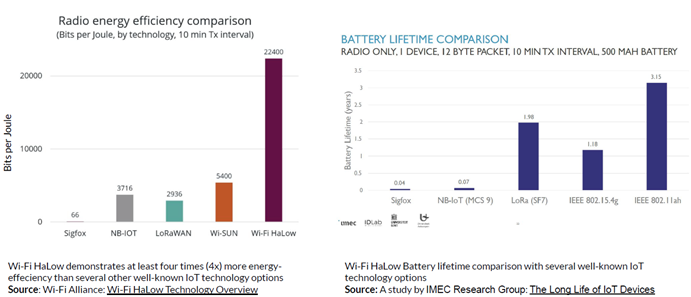
\includegraphics[width=0.8\textwidth]{images/WiFiEnergyEff.png}
    \caption{Сравнение энергоэффективности протоколов \cite{IMG_protocol_compare_power_eff}}
    \label{fig:wifi_energy_eff}
\end{figure}

\paragraph{Основные элементы архитектуры и топологии}
\begin{itemize}
  \item \textbf{Диапазон частот:} 863–928 МГц (региональные поддиапазоны).
  \item \textbf{Узлы:} 
    \begin{itemize}
      \item \emph{STA} (датчики/актуаторы) с поддержкой энергосбережения.
      \item \emph{AP} (Access Point) — единственный координатор сети, задаваемый при развертывании сети администратором.
      \item \emph{Relay AP} (опционально) — специальные узлы (ретрансляторы)
    \end{itemize}
  \item \textbf{Топология:} поддерживаются несколько вариантов: звездная и древовидная с ретрансляцией (ограниченное дерево без полного L2-mesh) для расширения до удалённых STA.
\end{itemize}

\paragraph{Преимущества и недостатки:}

В качестве преимуществ IEEE 802.11ah можно выделить большую дальность связи (до 3 км вне помещений при использовании ретранслятора Relay AP), высокую плотность подключений (возможность обслуживания сотен устройств одной точкой доступа), а также низкое энергопотребление при малой активности. Вместе с тем, стандарту присущи: низкая пропускная способность по сравнению с Wi-Fi в диапазонах 2,4/5/6 ГГц, более высокая сложность и стоимость модулей по сравнению с устройствами на базе 802.15.4, из-за чего данный протокол не получил широкого распространения среди потребительских устройств, заняв только небольшую нишу промышленных IoT-устройств; а также сложности лицензирования различных диапазонов частот для разных стран.
При отказе единственного AP вся BSS теряет синхронизацию и связь STA; стандарт не содержит механизмов внутреннего резервирования или автоматического фейловера.


%%%%%%%%%%%%%%%%%%%%%%%%%%%%%%%%%%%%%%%%%%%%%%%%%%%%%%%%%%%%%%%%%%%%%%%%%%%%%%%%%%%%%%%%%%%%%%%%%%%%%%%%%%%%%%%%%%%%%%%%%%%%%%%%%%%%%%%%%%%%%%%%%%%%%%%%%%%%%%%%%%%%%%%%%%%%%
%                                                                                                                                                                           %
%                                                                    BLUETOOTH AND BLUETOOTH LOW ENERGY                                                                     %
%                                                                                                                                                                           %
%%%%%%%%%%%%%%%%%%%%%%%%%%%%%%%%%%%%%%%%%%%%%%%%%%%%%%%%%%%%%%%%%%%%%%%%%%%%%%%%%%%%%%%%%%%%%%%%%%%%%%%%%%%%%%%%%%%%%%%%%%%%%%%%%%%%%%%%%%%%%%%%%%%%%%%%%%%%%%%%%%%%%%%%%%%%%
\subsubsection{Bluetooth Low Energy (BLE) и Bluetooth Mesh}

Bluetooth Low Energy (BLE) — низкоэнергетичная радиотехнология, оптимизированная для передачи небольших объёмов данных с минимальным расходом батареи и поддерживающая энергосберегающие
режимы. BLE определяет четыре базовые роли устройств: Central, Peripheral, Broadcaster и Observer, что позволяет строить радиосеть в топологии «Звезда» с центральным узлом (Central) и периферийными устройствами (Peripheral).
Частотный диапазон BLE включает 40 каналов в диапазоне 2,4–2,4835 ГГц: 37 каналов для передачи данных и 3 каналов для рекламы. Для масштабируемых IoT-решений существует расширение Bluetooth Mesh, позволяющее узлам ретранслировать
сообщения и формировать распределённую сеть «many-to-many» поверх BLE.

\paragraph{Роли устройств}
\begin{itemize}
  \item \textbf{Peripheral} — Энергоэффективное устройство, периодически транслирующее (advertise) данные и ждущее подключения от центрального узла (Central) \ref{fig:fig_BLE_topology_unicast}. Характерные примеры: пульсометры, датчики температуры, трекеры активности.
  \item \textbf{Central} — Стационарное устройство, выполняющее сканирование эфирных пакетов и устанавливающее соединения с одним или несколькими периферийными узлами. Часто это смартфоны, планшеты или концентраторы IoT--сетей, которым нужны данные от множества сенсоров.
  \item \textbf{Broadcaster} — Устройство с односторонней рекламой: без установления соединения периодически рассылает рекламные пакеты с полезной информацией (beacons) \ref{fig:fig_BLE_topology_broadcast}. Используется для вещания маячков близости, рекламных кампаний, навигации в помещениях (Indoor positioning system).
  \item \textbf{Observer} — Стационарное устройство-приёмник, которое пассивно сканирует эфир, собирая (несвязанную) информацию из рекламных пакетов Broadcaster’ов и Peripheral’ов. Применяется для мониторинга окружающей среды, подсчёта посетителей, сбора статистики о маячках.
\end{itemize}


\begin{figure}[htbp]
  \centering
  % Первая подфигура, выровнена по верху
  \begin{subfigure}[t]{0.45\textwidth}
    \centering
    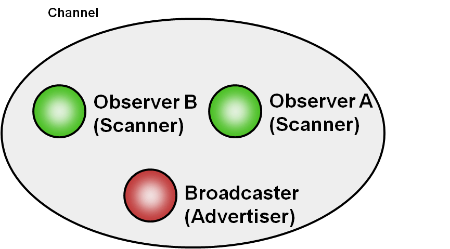
\includegraphics[width=\linewidth]{images/BLE-topology-broadcast.png}
    \caption{Broadcaster/Observer}
    \label{fig:fig_BLE_topology_broadcast}
  \end{subfigure}\hfill
  % Вторая подфигура, тоже по верху
  \begin{subfigure}[t]{0.45\textwidth}
    \centering
    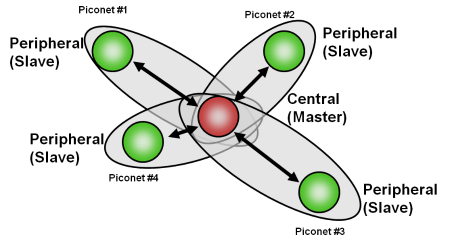
\includegraphics[width=\linewidth]{images/BLE-topology-unicast.png}
    \caption{Peripheral/Central}
    \label{fig:fig_BLE_topology_unicast}
  \end{subfigure}

  % Общая подпись
  \caption{Профили устройств BLE\cite{IMG_BLE_topologies}}
  \label{fig:twophotos}
\end{figure}



\paragraph{Применимость в системах автоматизации и IoT.}

BLE широко используется в умных домах, торговых и продуктовых центрах, медицине и иных сферах ИВ благодаря низкому энергопотреблению (десятки микроампер в спящем режиме) и широкой распространенности среди потребительских устройств.

\paragraph{BLE Mesh.}

Т.к. BLE Mesh лишь расширение стандарта, использующий особым образом режим рекламы для лавинообразного передачи сообщений, по техническим характеристикам он сильно похож на BLE.
Для поддержания совместимости было использовано лавинообразное рассылка (flooding \cite{BLE_mesh_spec}), которая с большим количеством устройств может значительно увеличить территорию
покрытия, но, с другой стороны, может привести к избыточной загруженности каналов, что после некоторой отметки в количестве устройств может привести к потерям пакетов.

%%%%%%%%%%%%%%%%%%%%%%%%%%%%%%%%%%%%%%%%%%%%%%%%%%%%%%%%%%%%%%%%%%%%%%%%%%%%%%%%%%%%%%%%%%%%%%%%%%%%%%%%%%%%%%%%%%%%%%%%%%%%%%%%%%%%%%%%%%%%%%%%%%%%%%%%%%%%%%%%%%%%%%%%%%%%%
%                                                                                                                                                                           %
%                                                                                 ZIGBEE                                                                                    %
%                                                                                                                                                                           %
%%%%%%%%%%%%%%%%%%%%%%%%%%%%%%%%%%%%%%%%%%%%%%%%%%%%%%%%%%%%%%%%%%%%%%%%%%%%%%%%%%%%%%%%%%%%%%%%%%%%%%%%%%%%%%%%%%%%%%%%%%%%%%%%%%%%%%%%%%%%%%%%%%%%%%%%%%%%%%%%%%%%%%%%%%%%%

\subsubsection{Zigbee и Zigbee Pro}

Стандарт ZigBee основан на IEEE~802.15.4 и работает в нелицензируемых ISM-диапазонах \cite{IEEE802_15_4_2020,ZIGBEE_SPEC_R23}: 2.4ГГц(глобально доступен и используется во всем мире), 915МГц (США, Канада, Австралия и Израиль).  868МГц (ЕC, Великобритания, Турция)

Области применения включают умные дома и городскую инфраструктуру, где используются системы управления освещением, датчики движения, решения для безопасности и “умные” счётчики в составе городских систем управления; промышленную автоматизацию с круглосуточным мониторингом состояния оборудования, предиктивным обслуживанием, сбором данных с вибрационных и температурных датчиков, дистанционным управлением приводами и оптимизацией технологических процессов; и медицинский мониторинг для удалённого сбора жизненных показателей пациентов и контроля заряда портативных медицинских устройств.

\paragraph{Основные элементы архитектуры и топологии}
\begin{itemize}
  \item \textbf{Узлы:} 
    \begin{itemize}
      \item \emph{Координатор (ZC)} единственный узел, создаёт PAN: сканирует каналы, выбирает свободный, задаёт PAN\_ID, Extended PAN\_ID, ключи безопасности, хранит таблицы маршрутизации и аутентификации.\newline Работает также как маршрутизатор.
      \item \emph{Маршрутизатор (ZR)} mains-powered, всегда активен, расширяет покрытие, ретранслирует пакеты, обеспечивает альтернативные пути.
      \item \emph{Конечное устройство (ZED)} battery-powered, не ретранслирует, общается только с родителем (координатором или маршрутизатором), включает режим сна.
    \end{itemize}
  \item \textbf{Топология:} ZigBee поддерживает три базовые топологии:
    \begin{itemize}
      \item \emph{Звёздная топология (Star)} Все узлы подключены непосредственно к координатору. Простая настройка, но ограничена радиусом и зависит от координатора.
      \item \emph{Деревовидная топология (Cluster-Tree)} Иерархия: координатор → маршрутизаторы уровней → конечные устройства. Адресация упрощена tree-адресацией, но узлы-маршрутизаторы становятся критическими точками.
      \item \emph{ячеистая топология (Mesh-network)} Любой маршрутизатор может ретранслировать пакет между любыми двумя узлами. Поддерживает самовосстановление при отказах и динамическое подключение новых устройств.
    \end{itemize}
\end{itemize}

Координатор задаётся программно администратором, но при запуске сети он автоматически:
\begin{itemize}
    \item сканирует каналы ISM;
    \item выбирает наименее загруженный канал;
    \item присваивает PAN\_ID;
    \item задаёт параметры: \texttt{NWK\_MAX\_CHILDREN}, \texttt{NWK\_MAX\_DEPTH}, \texttt{MAX\_ROUTERS}.
\end{itemize}

В сетях IEEE 802.15.4 с beacon-режимом координатор через равные интервалы от 15 мс до 4 минут рассылает фрейм-маяк, который объявляет начало очередного суперфрейма и указывает доступные слоты доступа\cite{IEEE802_15_4_2020}; обычно именно координатор является главным источником этих маяков, хотя в древовидных (cluster-tree) конфигурациях роль ретрансляторов могут брать на себя маршрутизаторы, тогда как в обычном mesh-режиме они маяки не посылают; при этом автоматическое резервирование источников маяков не предусмотрено, поэтому отказ узла-маяка приводит к потере синхронизации всей сети, и её приходится вручную восстанавливать.


\paragraph{Обнаружение маршрута} Процесс начинается с того, что узел-инициатор рассылает по сети широковещательный запрос на установление маршрута (RREQ), при этом указывается определённая метрика, например, количество переходов или качество канала.
Узел назначения, получив несколько RREQ от разных маршрутов, выбирает из них наиболее подходящий — согласно метрике — и отправляет одноадресный ответ (RREP) обратно к источнику, используя обратный путь, по которому был получен лучший запрос.

\paragraph{Передача и ретрансляция} После получения ответа (RREP) начинается передача данных. Информация передаётся от источника к получателю через промежуточные узлы. Каждый промежуточный узел проверяет свою таблицу маршрутизации, чтобы определить, куда направить пакет дальше, и ретранслирует пакет следующему узлу по цепочке.
Если ожидаемое подтверждение доставки (ACK) не поступает, инициируется сообщение об ошибке маршрута (RERR). В таком случае начинается повторное построение маршрута — запускается новый процесс рассылки RREQ.


\paragraph{Шаблоны устройств (Application Profiles)}
На уровне приложения Zigbee определяет профили устройств, что можнно наблюдать на рисунке \ref{fig:Zigbee_device_profile}:
\begin{itemize}
 \item \textbf{Публичные профили:} Home Automation, Commercial Building Automation и др.: лампы, выключатели, датчики, термостаты, розетки.
 \item \textbf{Частные профили:} Производители могут создавать собственные профили, но контроллер должен поддерживать их для взаимодействия.
\end{itemize}

Каждый профиль включает: \texttt{Profile ID}, \texttt{Device ID}, \texttt{Cluster IDs} и назначение энптойтов (адрес и адресат). Контроллер распознаёт и управляет устройством только при совпадении этих идентификаторов.


\begin{figure}[h]
    \centering
    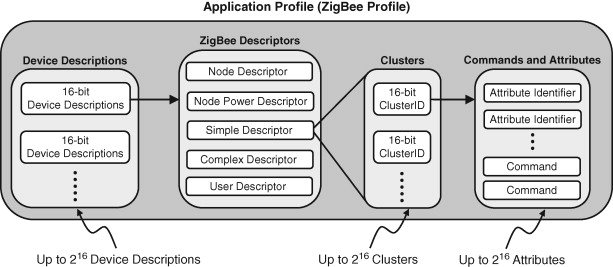
\includegraphics[width=0.8\textwidth]{images/Zigbee_device_profile.jpg}
    \caption{Профили устройств Zigbee \cite{IMG_Zigbee_profile}}
    \label{fig:Zigbee_device_profile}
\end{figure}

\paragraph{Влияние отказов}
\begin{itemize}
    \item \textbf{Координатор:} при его отказе сеть не функционирует, требует перезапуска с новым координатором \cite{Fault_Tolerance_ZigBee}.
    \item \textbf{Маршрутизатор:} потеря альтернативных путей, временная деградация доступности узлов, последующее самовосстановление \cite{Fault_Tolerance_ZigBee}.
    \item \textbf{Конечное устройство:} затрагивается только функционал этого узла, остальная сеть продолжает работу.
\end{itemize}

\paragraph{Zigbee Pro.}  

Zigbee Pro представляет собой расширенную реализацию базового протокола Zigbee, оптимизированную для высоконагруженных и масштабируемых сетей \cite{NXP_JNUG3101}. В отличие от классического Zigbee, Pro-версия обеспечивает поддержку сетей размером до нескольких тысяч узлов, более гибкую и самовосстанавливающуюся маршрутизацию, улучшенную управляющую функциональность (Many-to-One и Source Routing) и усиленные механизмы безопасности с отдельными ключами для транспортного и сетевого уровней.

В случае отказа координатора или маршрутизатора, сеть на базе Zigbee Pro демонстрирует лучшие возможности по сохранению связи и быстрому восстановлению работоспособности \cite{Fault_Tolerance_ZigBee} благодаря:
\begin{itemize}
  \item \textbf{Самовосстановлению маршрутов:} оставшиеся маршрутизаторы автоматически перестраивают таблицы маршрутов без участия центрального узла.
  \item \textbf{Source Routing и Many-to-One маршруты:} устройства могут кэшировать рабочие пути и переключаться на альтернативные узлы при недоступности основного, что снижает время простоя.
  \item \textbf{Гибкая архитектура Trust Center:} в Pro-режиме можно реализовать избыточные или внешние Trust Center (через облачные сервера или резервные координаторы), что позволяет продолжать авторизацию и обновление ключей даже при выходе из строя основного координатора.
\end{itemize}

Таким образом, выбор Zigbee Pro вместо «простого» Zigbee особенно оправдан в критичных системах, где недопустима потеря управляемости и долговременная деградация сети при отказах ключевых узлов.  


%%%%%%%%%%%%%%%%%%%%%%%%%%%%%%%%%%%%%%%%%%%%%%%%%%%%%%%%%%%%%%%%%%%%%%%%%%%%%%%%%%%%%%%%%%%%%%%%%%%%%%%%%%%%%%%%%%%%%%%%%%%%%%%%%%%%%%%%%%%%%%%%%%%%%%%%%%%%%%%%%%%%%%%%%%%%%
%                                                                                                                                                                           %
%                                                                           СРАВНЕНИЕ ПРОТОКОЛОВ                                                                            %
%                                                                                                                                                                           %
%%%%%%%%%%%%%%%%%%%%%%%%%%%%%%%%%%%%%%%%%%%%%%%%%%%%%%%%%%%%%%%%%%%%%%%%%%%%%%%%%%%%%%%%%%%%%%%%%%%%%%%%%%%%%%%%%%%%%%%%%%%%%%%%%%%%%%%%%%%%%%%%%%%%%%%%%%%%%%%%%%%%%%%%%%%%%


\subsubsection{Сравнение представленных протоколов}
На рис.~\ref{fig:protocols_range_vs_speed} представлен сравнительный график различных протоколов беспроводных сетей. Была составлена таблица~\ref{table:compare_wireless_protocols}.

\begin{figure}[h]
    \centering
    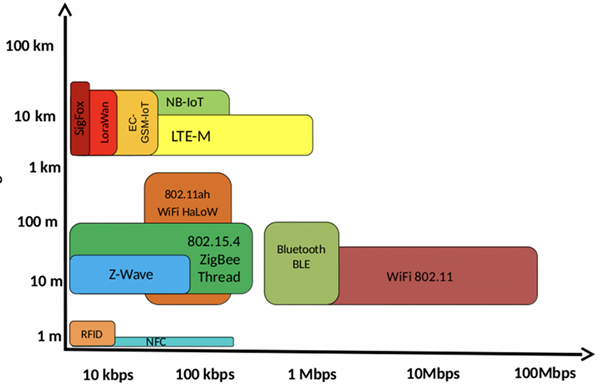
\includegraphics[width=0.8\textwidth]{images/Fig07.png}
    \captionsetup{justification=centering}
    \caption{Сравнение беспроводных протоколов передачи данных по дальности и скорости передачи. \cite{IMG_protocol_compare} }
    \label{fig:protocols_range_vs_speed}
\end{figure}


\paragraph{Wi-Fi}
Подходит, если устройства питаются от сети и требуют периодической двусторонней связи (настройка, диагностика), но энергопотребление высоко, а при отказе единственного роутера все «умные» приборы теряют соединение. Отсутствие готовых профилей усложняет быструю интеграцию простых сенсоров и актюаторов в экосистему без дополнительной логики на каждом устройстве.

\paragraph{Wi-Fi HaLow (802.11ah)}
Дает радиус работы в несколько сотен метров и низкое энергопотребление благодаря планируемым «пробуждениям», но требует специализированных модулей и ручной реализации логики таймингов и ретрансляции. Полезен для удалённых уличных датчиков, но не для систем автоматизации помещений.

\paragraph{BLE}
Идеален для маленьких беспроводных сенсоров: потребляет микроватты в спящем режиме, а «из коробки» доступно множество стандартизованных GATT-профилей (кнопки, переключатели, датчики температуры), что ускоряет выпуск простых устройств. Единственная точка сбора (смартфон или хаб) — SPOF, что незначительно при подключению к смартфону или ПК, но становится уязвимым местом при построении системы с большим количеством устройств.

\paragraph{BLE Mesh}
Устраняет SPOF за счёт децентрализованного flooding-ретранслятора, повышая надёжность покрытия, но сложность прошивки растёт: нужно описывать модели сообщений и управлять подписками, и батарейные устройства-ретрансляторы разряжаются быстрее.
Bluetooth Mesh не использует центрального координатора и строит сеть поверх классического BLE через управляемое «затопление» (managed flooding), что обеспечивает высокую отказоустойчивость и самовосстановление при выходе узлов из строя. В то же время это ведёт к повышенной сложности разработки (необходимость профилирования, управления ключами, времени-проживания сообщений и т. д.) и к компромиссам по энергоэффективности, решаемым с помощью ролей «низкоэнергетический узел»/«друг» (Low Power Node / Friend)

\paragraph{Zigbee}
Низкое энергопотребление и простая интеграция типовых устройств через ZCL-профилей (лампы, выключатели, датчики) делают его популярным в массовых установках. Однако жёстко централизованный PAN-Coordinator без автоматического резервирования превращает отключение хаба в полный отказ сети.

\paragraph{Zigbee Pro}
Добавляет самовосстановление mesh-маршрутов и резервирование Trust Center, что существенно повышает отказоустойчивость, сохраняя энергоэффективность и привычную модель ZCL-профилей. Разработка сложных нетиповых устройств усложняется из-за множества дополнительных опций маршрутизации и безопасности.

\paragraph{Thread}
Строит настоящий IPv6-mesh с динамическим лидером, без единой точки отказа, и самовосстанавливается через RPL. Отличается отличной надёжностью и низким потреблением сенсоров, но не предлагает «готовых» шаблонов устройств — для ламп и датчиков придётся проектировать обмен и структуру данных самостоятельно. Имеет высокий порог входа ввизу малой распространенности устройств для разработки (Dev-Kit).


\begin{table}[h!]
    \centering
    \renewcommand{\arraystretch}{1.3}
    \begin{tabularx}{\textwidth}{|X|X|X|X|}
        \hline
        \textbf{Имя} & \textbf{Пропускная способность} & \textbf{Дальность} & \textbf{Протокол маршрутизации} \\
        \hline
        Wi-Fi & до 23 Гбит/с & до 70 м в помещении и до 140 м на открытом местности & IEEE 802.11s (HWMP) \\
        \hline
        Wi-Fi HaLow & 150 Кбит/с – 347 Мбит/с & до 200 м в помещении и до 1 км на открытом местности & IEEE 802.11s (HWMP) \\
        \hline
        BLE Mesh & до 125 Кбит/с & до 100 м в помещении и до 300 м на открытой местности & Flooding \\
        \hline
        BLE Mesh & до 2 Мбит/с & до 400 м & managed flooding \\
        \hline
        Zigbee & до 250 Кбит/с & 10-100 м в помещении и 100–300 м на открытом местности & AODV (изменяемо) \\
        \hline
        Zigbee Pro & до 250 Кбит/с & 10–100 м в помещении и 100–300 м на открытом местности & AODV (изменяемо) \\
        \hline
        Thread & до 250 Кбит/с & 10–100 м в помещении и 100–300 м на открытом местности & MLE + distance-vector (RIPng) \\
        \hline
    \end{tabularx}
    \caption{Сравнительная таблица параметров беспроводных сетей}
    \label{table:compare_wireless_protocols}
\end{table}

\newpage

%%%%%%%%%%%%%%%%%%%%%%%%%%%%%%%%%%%%%%%%%%%%%%%%%%%%%%%%%%%%%%%%%%%%%%%%%%%%%%%%%%%%%%%%%%%%%%%%%%%%%%%%%%%%%%%%%%%%%%%%%%%%%%%%%%%%%%%%%%%%%%%%%%%%%%%%%%%%%%%%%%%%%%%%%%%%%
%%%%%%%%%%%%%%%%%%%%%%%%%%%%%%%%%%%%%%%%%%%%%%%%%%%%%%%%%%%%%%%%%%%%%%%%%%%%%%%%%%%%%%%%%%%%%%%%%%%%%%%%%%%%%%%%%%%%%%%%%%%%%%%%%%%%%%%%%%%%%%%%%%%%%%%%%%%%%%%%%%%%%%%%%%%%%
%%%%%%%%%%%%%%%%%%%%%%%%%%%%%%%%%%%%%%%%%%%%%%%%%%%%%%%%%%%%%%%%%%%%%%%%%%%%%%%%%%%%%%%%%%%%%%%%%%%%%%%%%%%%%%%%%%%%%%%%%%%%%%%%%%%%%%%%%%%%%%%%%%%%%%%%%%%%%%%%%%%%%%%%%%%%%
%                                                                                                                                                                           %
%                                                                   ГЛАВА II. Общее описание системы                                                                        %
%                                                                                                                                                                           %
%%%%%%%%%%%%%%%%%%%%%%%%%%%%%%%%%%%%%%%%%%%%%%%%%%%%%%%%%%%%%%%%%%%%%%%%%%%%%%%%%%%%%%%%%%%%%%%%%%%%%%%%%%%%%%%%%%%%%%%%%%%%%%%%%%%%%%%%%%%%%%%%%%%%%%%%%%%%%%%%%%%%%%%%%%%%%
%%%%%%%%%%%%%%%%%%%%%%%%%%%%%%%%%%%%%%%%%%%%%%%%%%%%%%%%%%%%%%%%%%%%%%%%%%%%%%%%%%%%%%%%%%%%%%%%%%%%%%%%%%%%%%%%%%%%%%%%%%%%%%%%%%%%%%%%%%%%%%%%%%%%%%%%%%%%%%%%%%%%%%%%%%%%%
%%%%%%%%%%%%%%%%%%%%%%%%%%%%%%%%%%%%%%%%%%%%%%%%%%%%%%%%%%%%%%%%%%%%%%%%%%%%%%%%%%%%%%%%%%%%%%%%%%%%%%%%%%%%%%%%%%%%%%%%%%%%%%%%%%%%%%%%%%%%%%%%%%%%%%%%%%%%%%%%%%%%%%%%%%%%%


\section{Глава 2. Общее описание системы}

\subsection{Проблемы, решаемые предлагаемой системой}

Система домашней автоматизации, осуществляющие обработку сценариев при помощи облачных сервисов либо с помощью центра умного дома, обладай несомненными преимуществами, такими как
простота настройки и реализации также имеют ряд недостатков.
\begin{enumerate}
\item \textbf{Высокая задержка:} Cобытие, поступающее от сенсора должно пройти длинный путь от устройства инициатора к центру умного
дома, пройти обработку и быть передано в виде команды устройству актуатору. Использование шаблонов устройств позволяет упростить взаимодействие сенсоров и актуаторов в системе, так,
например, системы использующие ZigBee могут устанавливать соединение напрямую между некоторыми устройствами используя технологию binding \cite{ZIGBEE_SPEC_R23}. Такой подход может существенно
снизить нагрузку на координатор сети и ретрансляторы, но не решает проблему сложных взаимодействий. Также данный метод предполагает использование однотипных шаблонов из-за чего
устройство разных производителей зачастую всё-таки будут взаимодействовать через центр умного дома.
\item \textbf{Отказоустойчивость:} Использование центра умного дома либо облачные инфраструктуры для обработки сценариев потенциально снижает надёжность системы: отказ
централизованного обработчика парализует работу СДА. Использование кадров маяка для синхронизации также вностит ограничение на отказоустойчивость системы: выход из строя координатора,
задающего синхронизационный фрейм также парализует СДА.
\end{enumerate}

\subsection{Предлагаемые нововведения}

Предлагаемый набор нововведений, позволяющих решить список потенциальных проблем:
\begin{enumerate}
\item Перенос обработки логики событий из центра умного дома (или облачного сервиса) в устройства-актуаторы.
\item Для взаимодействия устройств предлагается использование паттерна <<наблюдатель>> (Subject-Observer).
\item Для объединения устройств из разных локаций в единую сеть предлагается использование распределённого отказаустойчивого кластера, выполняющего
функции моста (ретрансляция сообщений внутри сети) и координатора сети (настройки системы, добавление и удаление устройств) и позволяющего удаленно управлять и отслеживать состояние
умного дома. Предполагается использование минимум одного узла кластера в каждой локации. На рис.~\ref{fig:GlobalSystemDesing} представлена архитектура предлагаемой гибридной системы.
\item С целью повышения отказоустойчивости предлагается использование CSMA \cite{CSMA_article} для предотвращения коллизии сообщений и отказа от фрейма синхронизации.
\end{enumerate}


\begin{figure}[h]
    \centering
    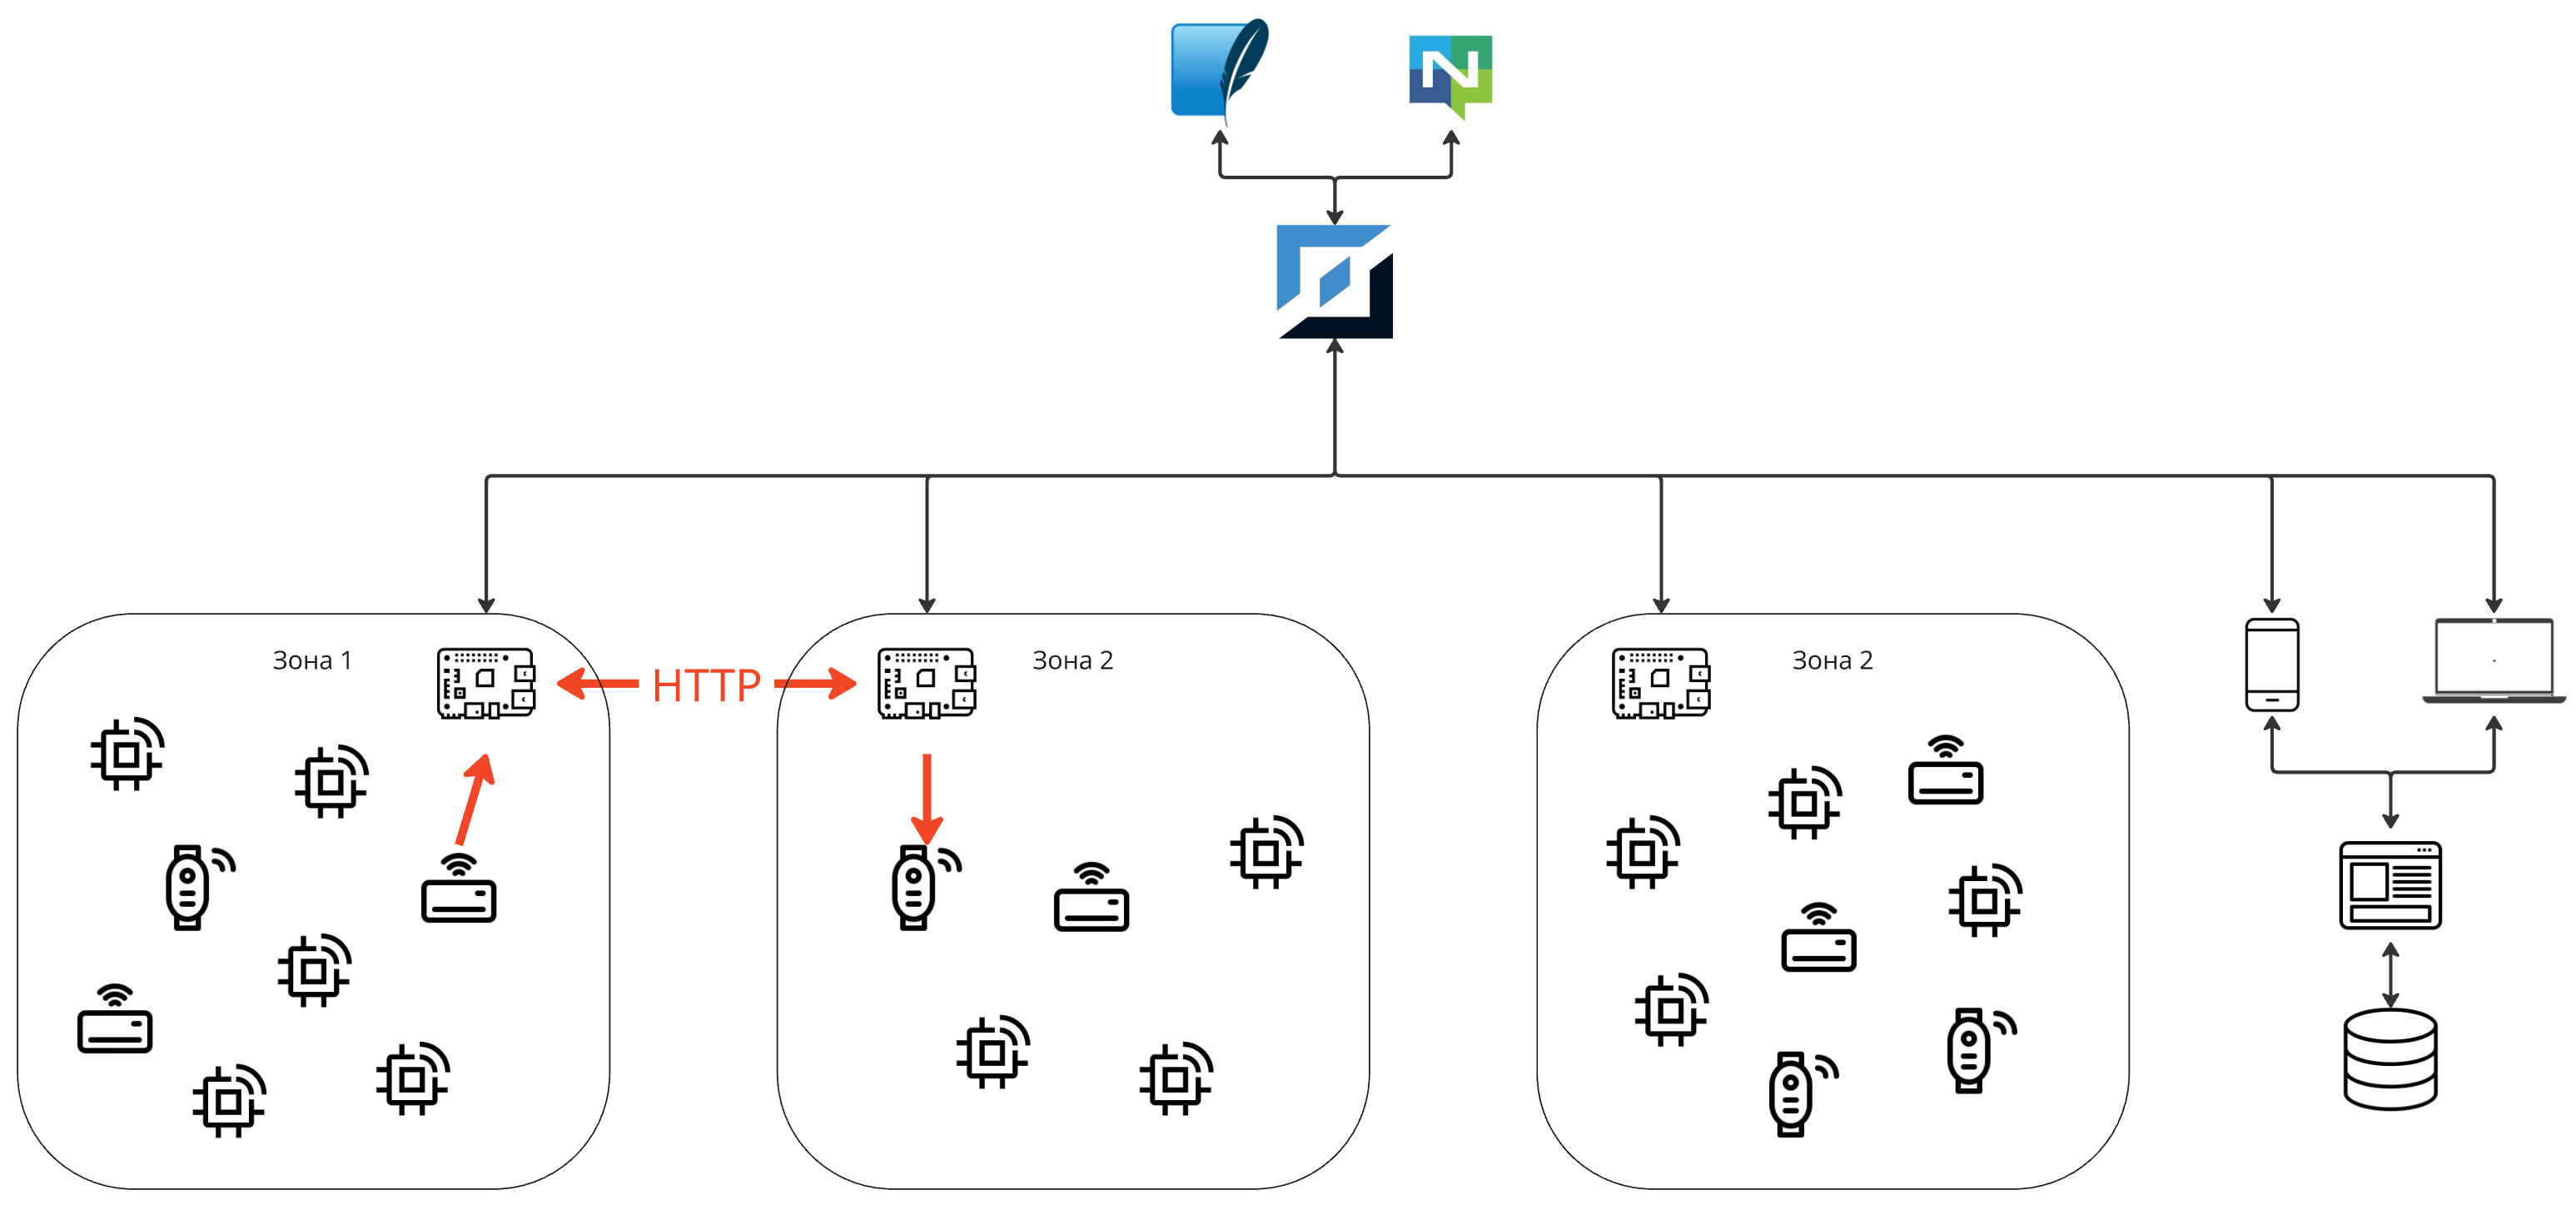
\includegraphics[width=0.8\textwidth]{images/GlobalSystemDesing.png}
    \caption{Пример СДА с распределенной структурой}
    \label{fig:GlobalSystemDesing}
\end{figure}

\subsection{Обоснование нововведений}

Данный подход позволит снизить задержки, так как вдвое сокращается количество передаваемых сообщений в режиме one-to-one и в n раз в случае передачи сообщений one-to-many. Также
снижение задержек происходит в виду отсутствие необходимости поочередной передачи команд каждому устройству, если событие подразумевает одновременное взаимодействие нескольких
устройств, например, по нажатию выключателя включение группы ламп. Данное решение также повышает отказоустойчивость сети из-за отсутствия промежуточных узлов: надёжность системы
зависит только от надёжности устройства-сенсора и устройства-актуатора, а в случае использования межзональных сценариев также от узлов кластера из этих локаций.

Использование CSMA хоть и приводит к чуть большему потреблению стационарных устройств, но позволяет отказаться от генератора синхронизирующих фреймов, которым обычно выступает
координатор сети. В таком случае выход из строя координатора либо его отключение ограничиться только невозможностью удалять добавлять и переконфигурировать сеть но не скажется на работоспособности сети

Данное решение кроме повышения надежности системы также уменьшает задержку передачи информации, повышает отказоустойчивость системы и ее безопасность \cite{SecuritySmartHome, SecuritySmartHome2}.


%%%%%%%%%%%%%%%%%%%%%%%%%%%%%%%%%%%%%%%%%%%%%%%%%%%%%%%%%%%%%%%%%%%%%%%%%%%%%%%%%%%%%%%%%%%%%%%%%%%%%%%%%%%%%%%%%%%%%%%%%%%%%%%%%%%%%%%%%%%%%%%%%%%%%%%%%%%%%%%%%%%%%%%%%%%%%
%%%%%%%%%%%%%%%%%%%%%%%%%%%%%%%%%%%%%%%%%%%%%%%%%%%%%%%%%%%%%%%%%%%%%%%%%%%%%%%%%%%%%%%%%%%%%%%%%%%%%%%%%%%%%%%%%%%%%%%%%%%%%%%%%%%%%%%%%%%%%%%%%%%%%%%%%%%%%%%%%%%%%%%%%%%%%
%%%%%%%%%%%%%%%%%%%%%%%%%%%%%%%%%%%%%%%%%%%%%%%%%%%%%%%%%%%%%%%%%%%%%%%%%%%%%%%%%%%%%%%%%%%%%%%%%%%%%%%%%%%%%%%%%%%%%%%%%%%%%%%%%%%%%%%%%%%%%%%%%%%%%%%%%%%%%%%%%%%%%%%%%%%%%
%                                                                                                                                                                           %
%                                                              ГЛАВА III. Конечные устройства.                                                                   %
%                                                                                                                                                                           %
%%%%%%%%%%%%%%%%%%%%%%%%%%%%%%%%%%%%%%%%%%%%%%%%%%%%%%%%%%%%%%%%%%%%%%%%%%%%%%%%%%%%%%%%%%%%%%%%%%%%%%%%%%%%%%%%%%%%%%%%%%%%%%%%%%%%%%%%%%%%%%%%%%%%%%%%%%%%%%%%%%%%%%%%%%%%%
%%%%%%%%%%%%%%%%%%%%%%%%%%%%%%%%%%%%%%%%%%%%%%%%%%%%%%%%%%%%%%%%%%%%%%%%%%%%%%%%%%%%%%%%%%%%%%%%%%%%%%%%%%%%%%%%%%%%%%%%%%%%%%%%%%%%%%%%%%%%%%%%%%%%%%%%%%%%%%%%%%%%%%%%%%%%%
%%%%%%%%%%%%%%%%%%%%%%%%%%%%%%%%%%%%%%%%%%%%%%%%%%%%%%%%%%%%%%%%%%%%%%%%%%%%%%%%%%%%%%%%%%%%%%%%%%%%%%%%%%%%%%%%%%%%%%%%%%%%%%%%%%%%%%%%%%%%%%%%%%%%%%%%%%%%%%%%%%%%%%%%%%%%%
\newpage

\section{Глава 3. Конечные устройства.}

\subsection{Аппаратная реализация конечных устройств.}

\subsubsection{Обоснование выбора аппаратной платформы}

В качестве аппаратной платформы конечных устройств системы домашней автоматизации выбран микроконтроллер STM32F411 семейства STM32 (STMicroelectronics). Данное семейство отличается
высоким уровнем интеграции, широкой линейкой моделей, а также возможностью масштабирования — от энергоэффективных решений до высокопроизводительных микроконтроллеров. В частности,
совместимость пинов питания и некоторых интерфейсов (UART, SPI, I²C, ADC, и др.) между различными линейками (STM32F0, F1, F3, F4 и др.) позволяет замену микросхем без необходимости
внесения значительных изменений в схемотехническое решение.

Выбор серии STM32F4 обусловлен необходимостью выполнения интерпретируемого кода на конечных устройствах. В частности, в рамках данного проекта планировался запуск встроенного
JavaScript-интерпретатора, который требует наличия значительного объёма оперативной памяти (не менее 64 КБ ОЗУ) и производительного ядра. STM32F411 с ядром Cortex-M4 и 128/256 КБ
ОЗУ полностью удовлетворяет данным требованиям, при этом оставаясь относительно доступным и распространённым решением.

Дополнительным фактором при выборе аппаратной платформы послужила возможность разработки в среде Arduino IDE. В отличие от STM32WB, обеспечивающего полноценную поддержку беспроводных
протоколов Zigbee и Thread, STM32F411 может быть полноценно использован в Arduino-среде через STM32duino core. Это особенно важно в условиях ограничения времени и необходимости
быстрой интеграции: в рамках проекта приоритетом была высокая скорость разработки и наличие широкого сообщества, предоставляющего библиотеки, примеры и поддержку. Разработка через
STM32CubeIDE или использование HAL/LL библиотек требует существенно более высокого порога вхождения, что снижает доступность технологии для разработчиков с опытом, ограниченным
Arduino-экосистемой.

\subsubsection{Обоснование выбора радиомодуля}

В качестве радиомодуля выбран микросхема SI4432 производства Silicon Labs. Данный модуль обеспечивает надёжную и энергоэффективную радиосвязь в диапазоне 433/868/915 МГц с высокой
чувствительностью приёмника (до –121 дБм) и выходной мощностью до +20 дБм, что позволяет обеспечить устойчивую связь на больших расстояниях и в условиях радиопомех. Немаловажным
преимуществом является буфера сообщений объемомо 64Б, что является самым большим показателем, среди радиомодулей-претендентов. Также при выборе ключевым аспектом выбора радиомодуля
была его интеграция в универсальную библиотеку беспроводной связи для встраиваемых устройств RadioLib.

Хотя Zigbee (в частности, Zigbee Pro) признан промышленным стандартом для реализации распределённых систем автоматизации, включая системы «умного дома», его внедрение в рамках Arduino
IDE представляется затруднительным. В частности, несмотря на наличие Zigbee-совместимых микроконтроллеров семейства STM32WB, полноценная работа с данным протоколом требует
использования STM32CubeWB~SDK и разработки в STM32CubeIDE, что влечёт за собой необходимость освоения принципиально иной среды и подхода разработки. Поддержка Zigbee в
рамках STM32duino отсутствует, а готовых библиотек для Arduino IDE расширяющих функционал STM32duino нет.

Использование радиомодуля SI4432 позволяет реализовать собственный стек передачи данных, гибко настраиваемый под конкретные требования проекта. Несмотря на необходимость разработки
протокольного уровня связи, данный подход обеспечивает более высокую скорость разработки, по сравнению с использованием STM32CubeWB~SDK.

\subsubsection{Проектирование конечного устойства.}

В среде проектирования электронных схем EasyEDA была разработана принципиальная схема устройства, представленная на рисунке~\ref{fig:STM32_schematic}. В той же среде выполнена
трассировка печатной платы. Изготовление платы осуществлено по лазерно-утюжной технологии (ЛУТ), обеспечивающей высокую точность и преемлемое качество получаемого рисунка проводников.

\begin{figure}[H]
    \centering
    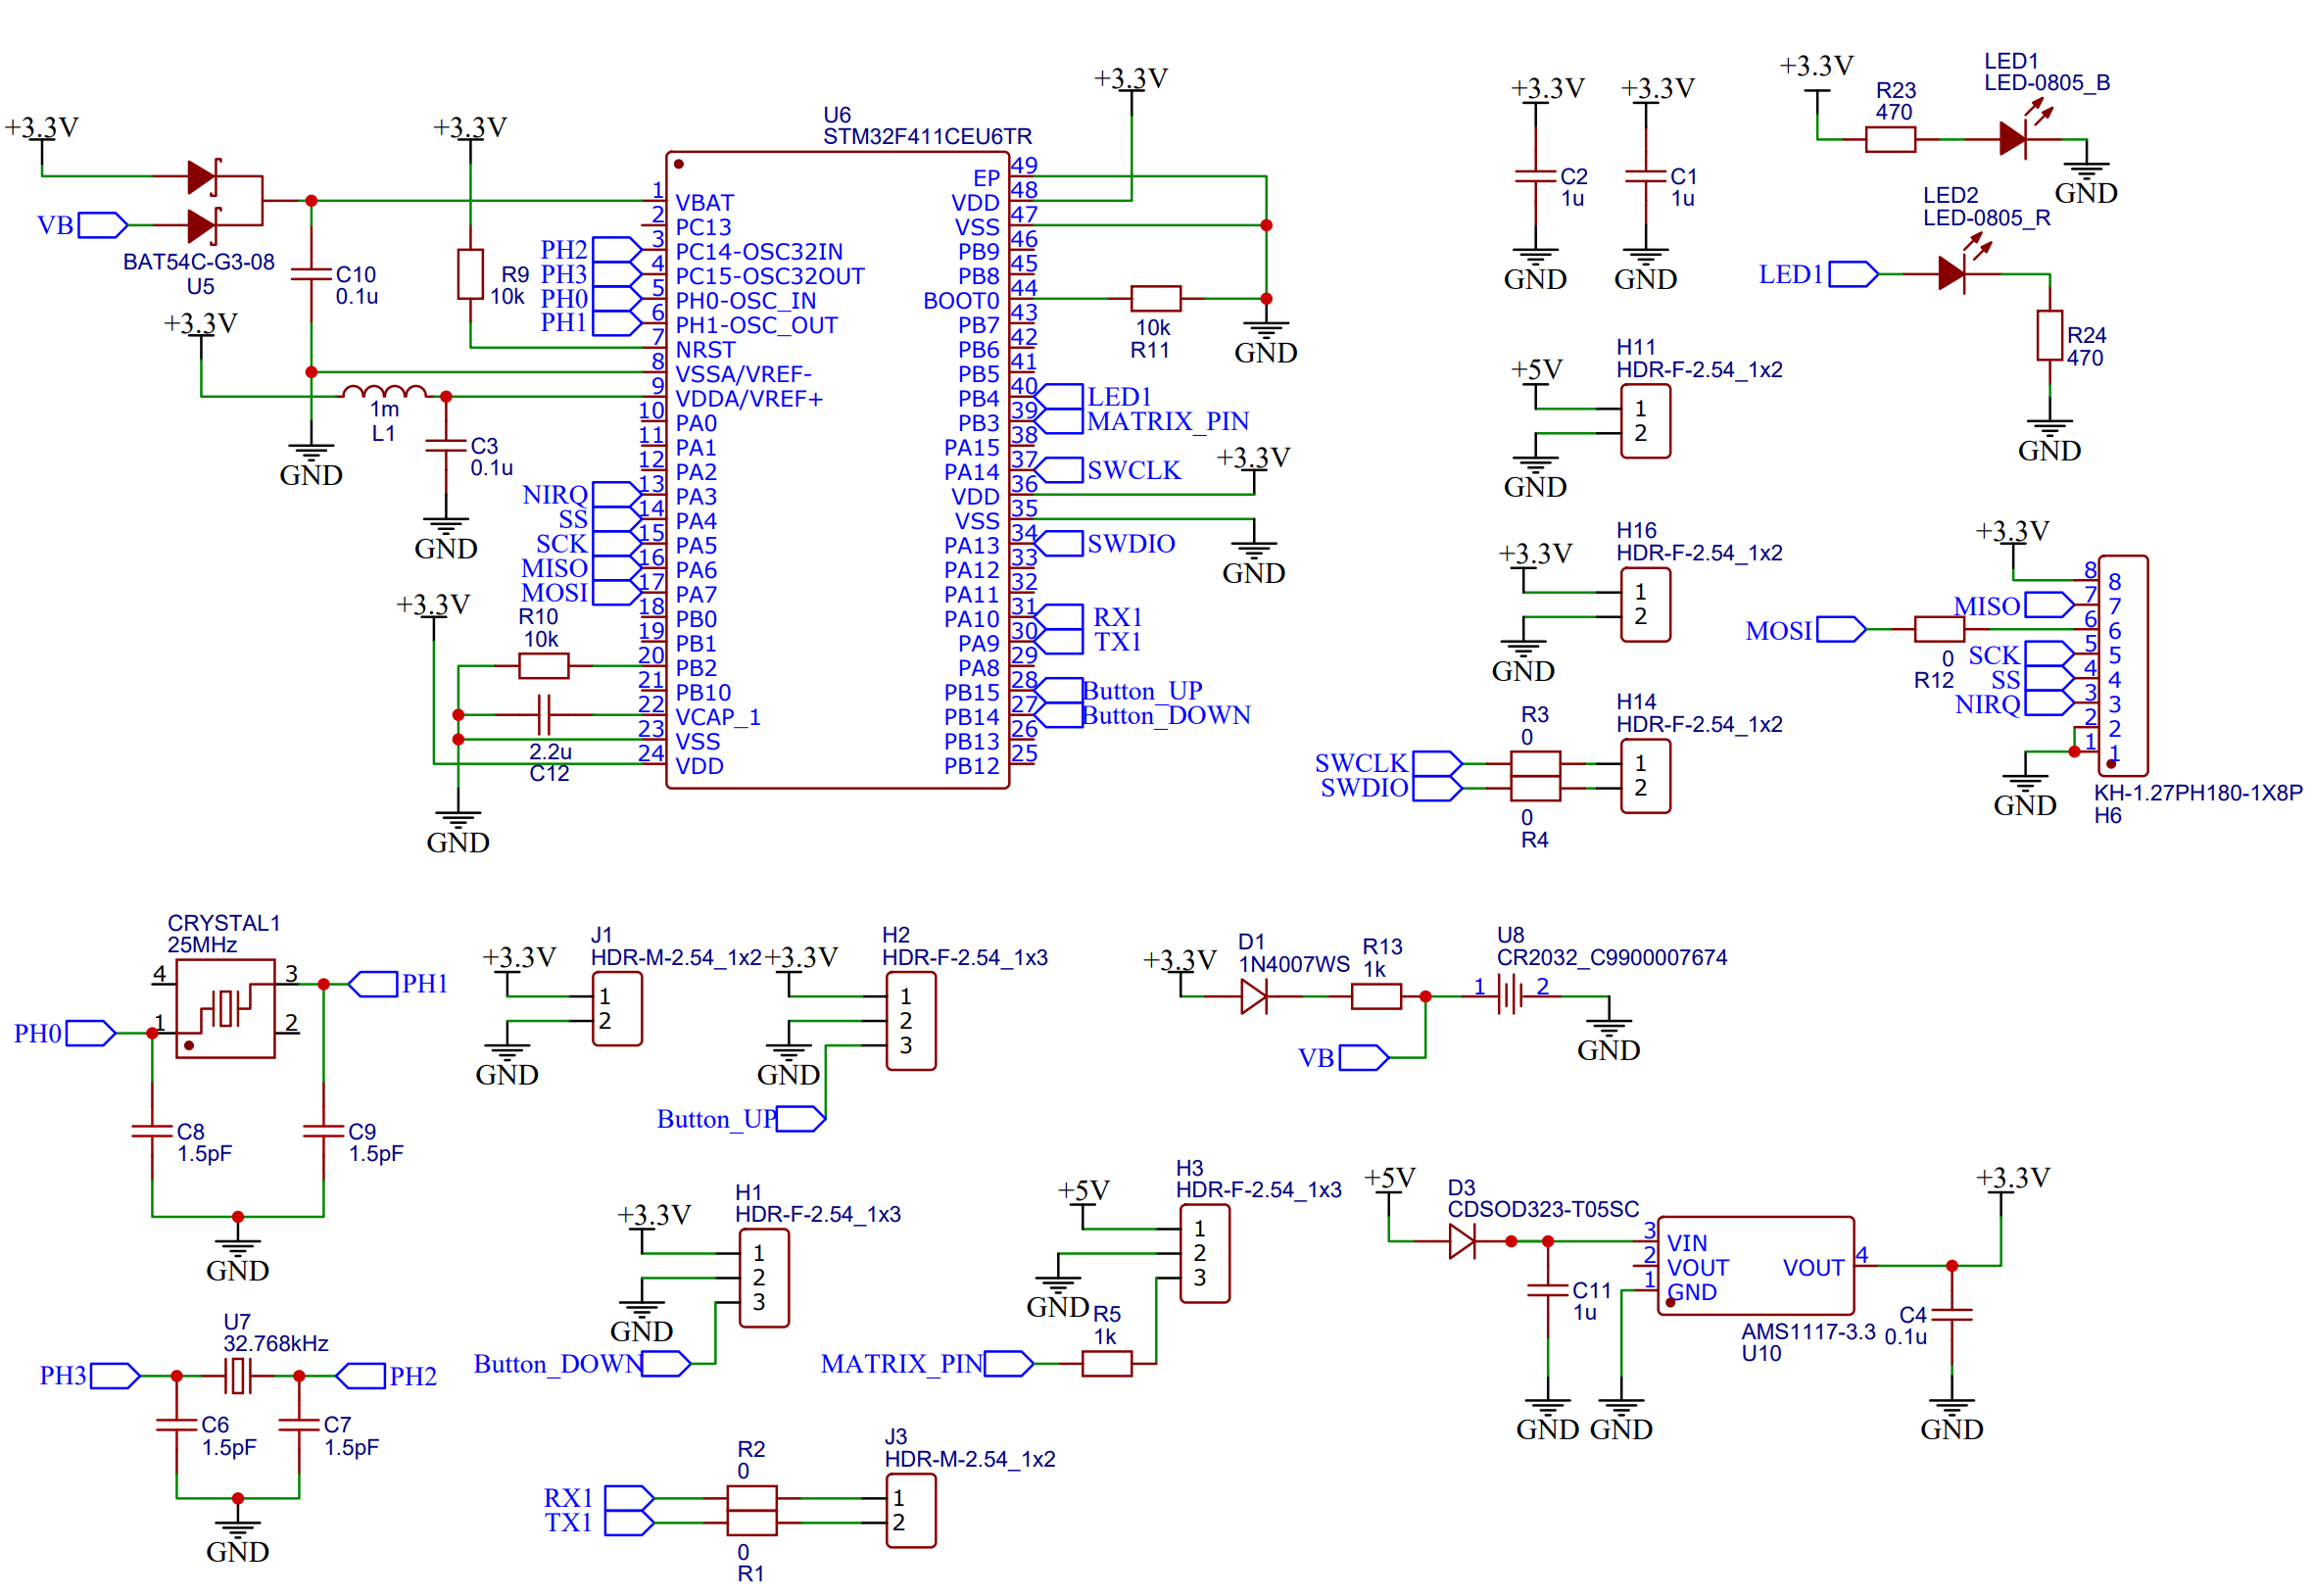
\includegraphics[width=0.8\textwidth]{images/STM32_schematic.png}
    \caption{Принципиальная схема устройства}
    \label{fig:STM32_schematic}
\end{figure}

После изготовления платы проведён монтаж электронных компонентов, включающий установку и пайку всех элементов в соответствии с разработанной схемой. Готовая плата прошла тестирование
на наличие коротких замыканий и обрывов дорожек с целью обеспечения её функциональной надёжности.

Программирование и отладка микроконтроллера на плате осуществлялись с использованием устройства WeAct Mini Debugger -- компактного программатора -- отладчика, поддерживающего протокол
StLink 2.1 для программирования микроконтроллеров STM32 и подключающегося к компьютеру через USB--порт.


%%%%%%%%%%%%%%%%%%%%%%%%%%%%%%%%%%%%%%%%%%%%%%%%%%%%%%%%%%%%%%%%%%%%%%%%%%%%%%%%%%%%%%%%%%%%%%%%%%%%%%%%%%%%%%%%%%%%%%%%%%%%%%%%%%%%%%%%%%%%%%%%%%%%%%%%%%%%%%%%%%%%%%%%%%%%%
%                                                                                                                                                                           %
%                                                               Программная реализация конечных устройств                                                                   %
%                                                                                                                                                                           %
%%%%%%%%%%%%%%%%%%%%%%%%%%%%%%%%%%%%%%%%%%%%%%%%%%%%%%%%%%%%%%%%%%%%%%%%%%%%%%%%%%%%%%%%%%%%%%%%%%%%%%%%%%%%%%%%%%%%%%%%%%%%%%%%%%%%%%%%%%%%%%%%%%%%%%%%%%%%%%%%%%%%%%%%%%%%%

\subsection{Программное обеспечение конечных устройств.}

Для обеспечения минимальных задержек и надёжного выполнения разнообразных задач на однокристальном контроллере STM32F411 применяется операционная система реального времени FreeRTOS,
интегрированная через STM32Duino. Архитектура FreeRTOS основана на ядре планировщика, которое управляет созданными задачами (tasks), их приоритетами и выделением ресурсов процессорного
времени и оперативной памяти (см. рисунок~\ref{fig:simple_arch_of_FreeRTOS}). Каждая задача располагает собственным стеком и может быть настроена на срабатывание по программируемому
таймеру, что позволяет гарантировать её запуск через заданные интервалы времени. Планировщик FreeRTOS реализует приоритетный вытесняющий (preemptive) режим: если текущая задача
превысила выделённый ей квант или в систему добавилась задача более высокого приоритета, управление незамедлительно передаётся вновь приоритетной задаче. Такая модель обеспечивает
детерминированное поведение и высокую отзывчивость конечного устройства.

\begin{figure}[H]
    \centering
    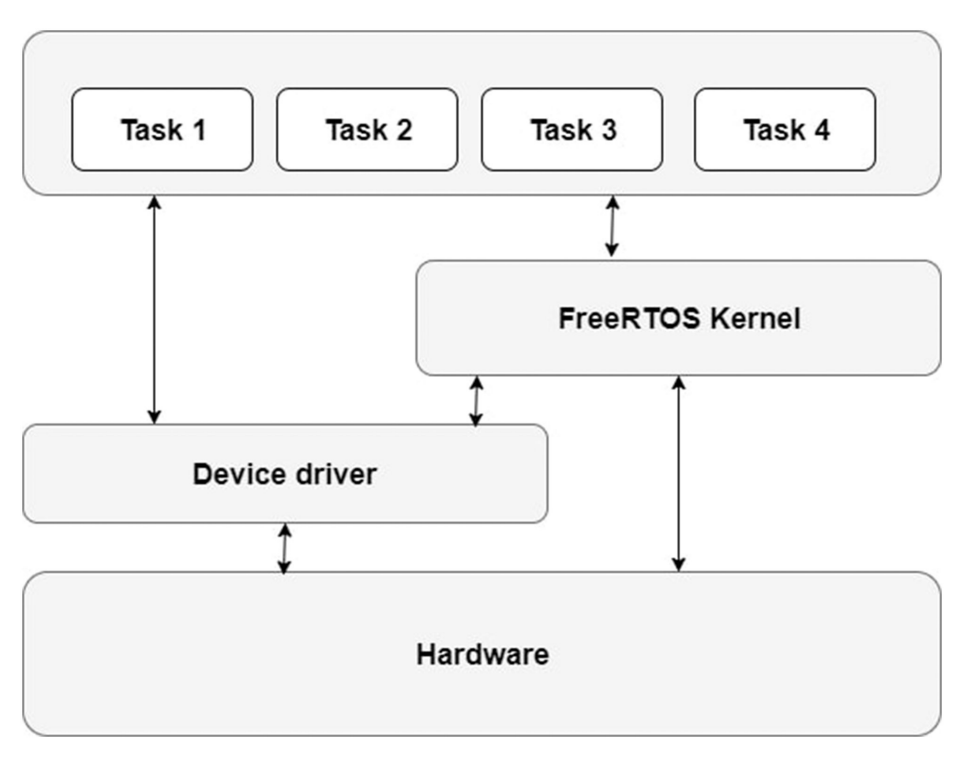
\includegraphics[width=0.8\textwidth]{images/FreeRTOS_arch.png}
    \caption{Упрощенная архитектура FreeRTOS \cite{IMG_RTOS_architectures}}
    \label{fig:simple_arch_of_FreeRTOS}
\end{figure}

Для повышения отказоустойчивости и сокращения времени обработки входящих сообщений отправка и приём сообщений разбиты на множество мелких задач, каждая из которых выполняет строго
определённый фрагмент обработки. Например, непосредственно чтение очередного пакета из буфера радиомодуля SI4432 обладает самым высоким приоритетом, затем следует проверка целостности
данных и, лишь после этого, формирование отладочных сообщений на последовательный порт — см. рисунок \ref{fig:STM32_architecture_of_messanger}. Подобное разделение предотвращает
«залипание» конвейера обработки и минимизирует вероятность образования битых пакетов.

\begin{figure}[H]
    \centering
    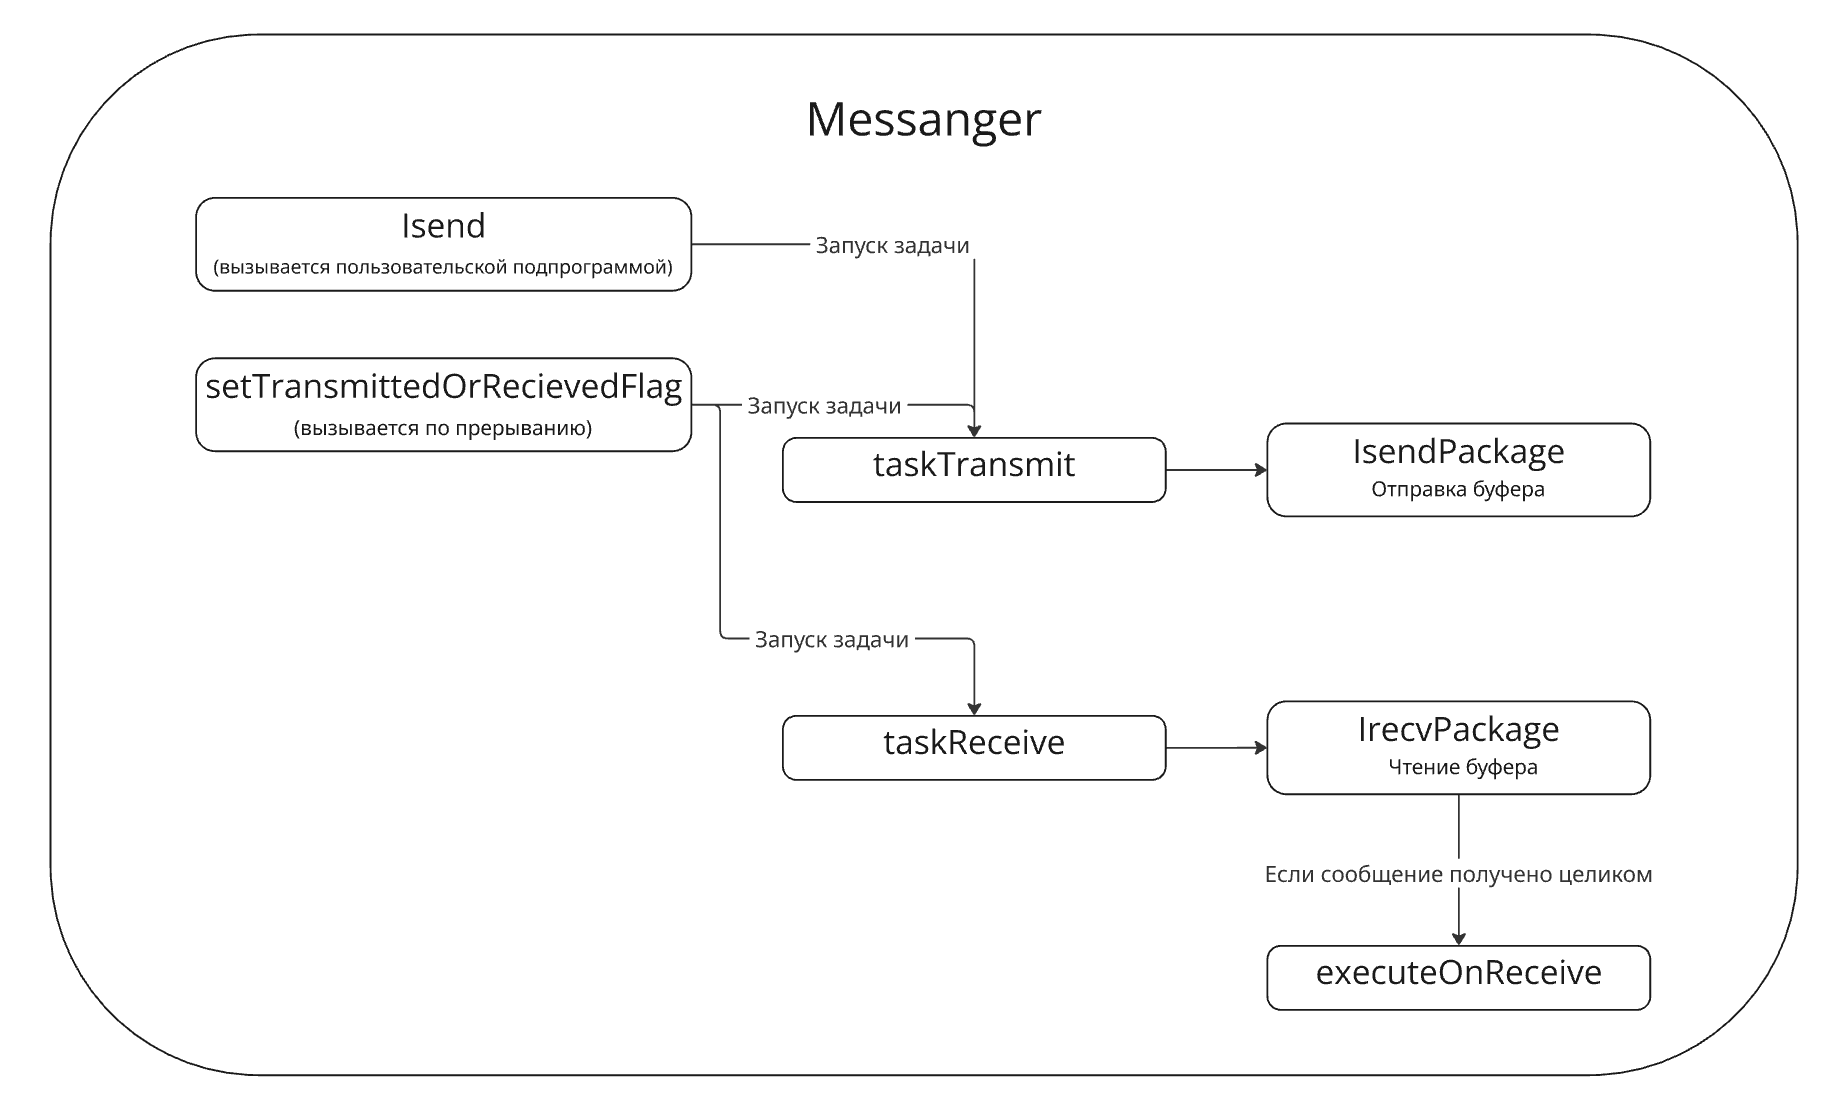
\includegraphics[width=0.8\textwidth]{images/Task_interaction.png}
    \caption{Упрощенное взаимодействие задач в библиотеке Messanger}
    \label{fig:STM32_architecture_of_messanger}
\end{figure}

Программная структура конечного устройства выстроена по двухуровневой схеме (рис. \ref{fig:end_device}). Низкоуровневая прошивка, написанная на C/C++ с использованием STM32Duino и FreeRTOS, предоставляет API для всех аппаратно-зависимых операций: настройка периферии, обмен данными с радиомодулем, синхронизация задач и работа с очередями сообщений. Высокоуровневая прошивка реализована на языке JavaScript и исполняется на встроенном интерпретаторе (например, JerryScript). Такая двухслойная архитектура позволяет оперативно изменять логику работы устройства без перепрошивки микроконтроллера: достаточно обновить JavaScript-модули через удалённую конфигурацию. Пакетный режим передачи сообщений с гибкими настройками параметров радиомодуля SI4432 доказал свою эффективность при прототипировании, сочетая низкое потребление энергии с высокой скоростью и надёжностью связи.

\begin{figure}[H]
    \centering
    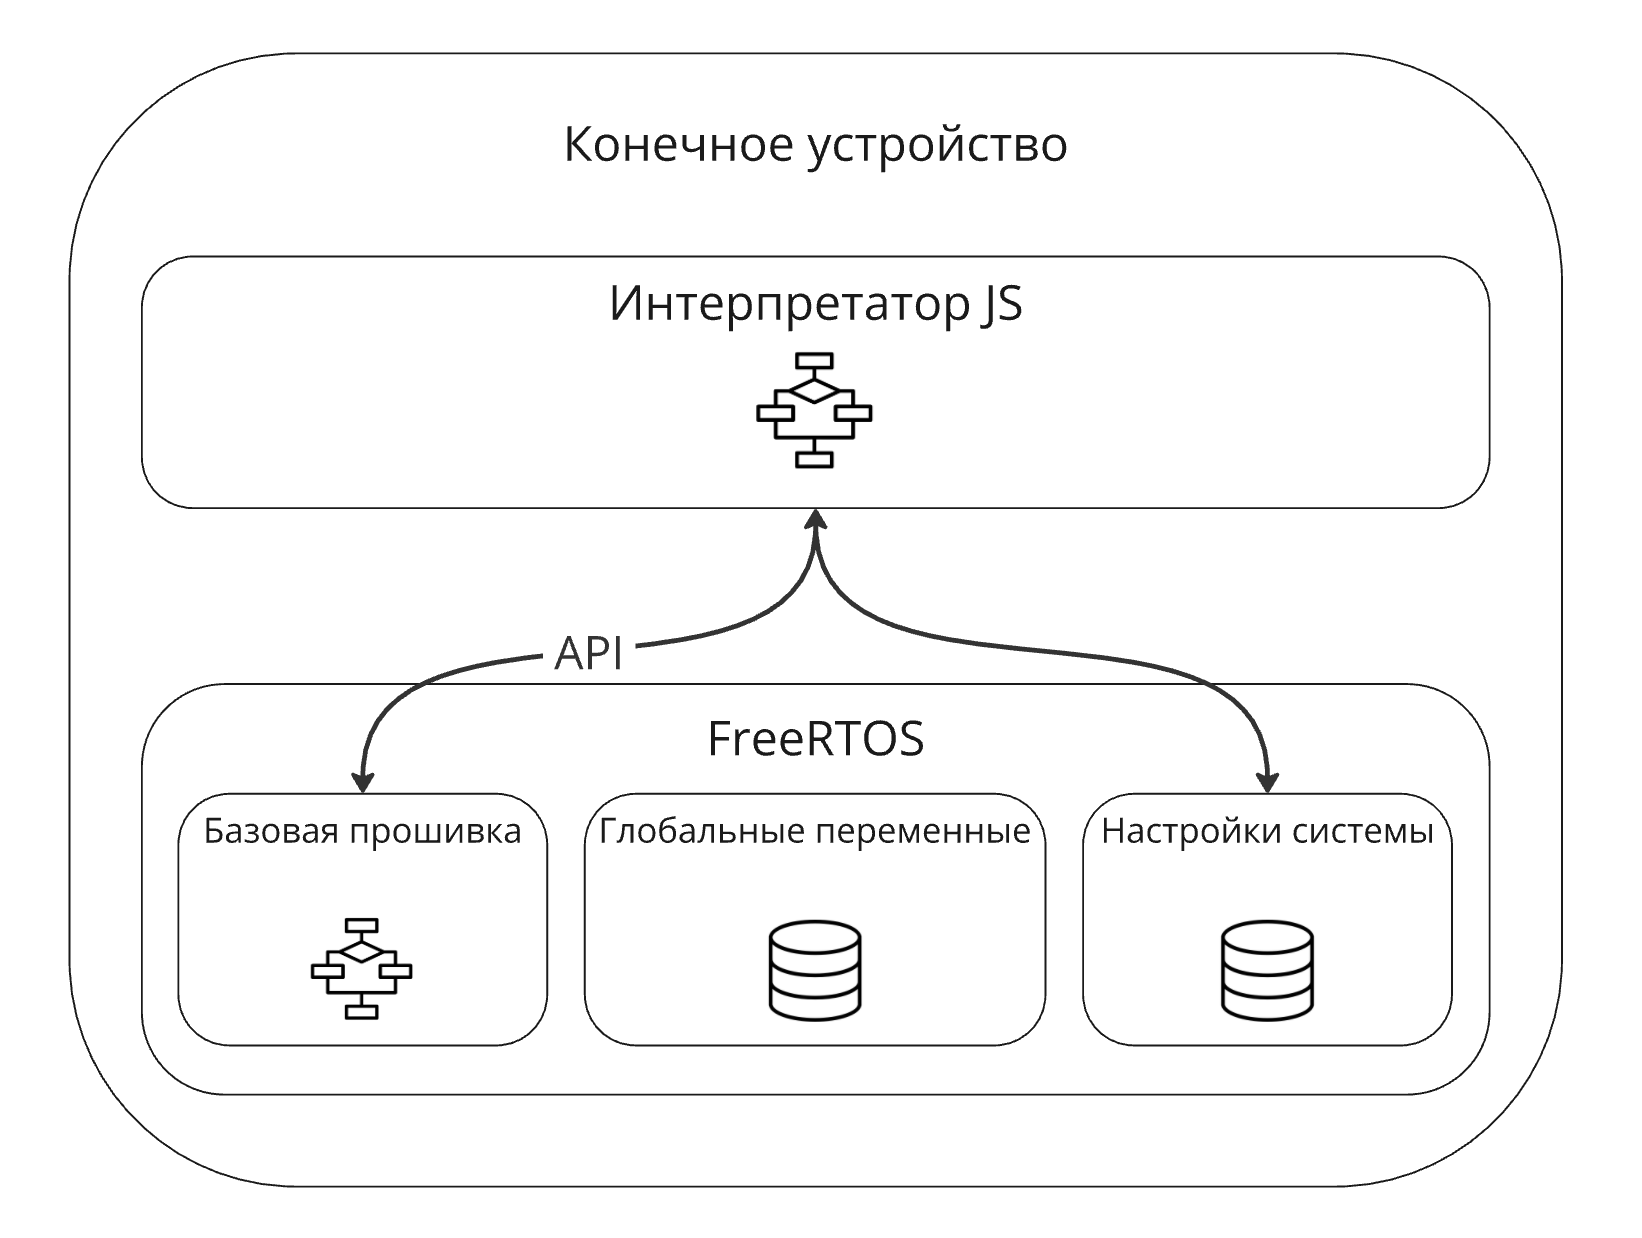
\includegraphics[width=0.8\textwidth]{images/Fig05.png}
    \caption{Реализация конечного устройства}
    \label{fig:end_device}
\end{figure}

\subsubsection{Интерпретатор JavaScript}

TinyJS представляет собой компактный (приблизительно 2000 строк кода) интерпретатор JavaScript, реализованный на C++ без внешних зависимостей, что обеспечивает простую интеграцию
в проекты для микроконтроллеров. Он поддерживает работу с переменными, массивами и структурами, функции (включая передачу параметров и возврат значений), а также встроенные механизмы
разбора и генерации JSON. Интерпретатор допускает вызов C/C++ кода из скриптов и обеспечивает базовую модель объектов с наследованием; выполнение производится напрямую из исходного
текста с помощью рекурсивного нисходящего парсера. Благодаря отсутствию промежуточной компиляции и минимальному объёму кода TinyJS удобно использовать для настройки параметров,
автоматизации простого поведения и загрузки/сохранения конфигураций на устройствах с ограниченными ресурсами. Несмотря на то, что проект не претендует на полное соответствие стандарту
ECMAScript и не оптимизирован для интенсивных вычислений, его лёгкая архитектура позволяет встраивать интерпретатор в микроконтроллерные платформы с достаточным объёмом оперативной
памяти.


%%%%%%%%%%%%%%%%%%%%%%%%%%%%%%%%%%%%%%%%%%%%%%%%%%%%%%%%%%%%%%%%%%%%%%%%%%%%%%%%%%%%%%%%%%%%%%%%%%%%%%%%%%%%%%%%%%%%%%%%%%%%%%%%%%%%%%%%%%%%%%%%%%%%%%%%%%%%%%%%%%%%%%%%%%%%%
%                                                                                                                                                                           %
%                                                                        Модель взаимодействия устройств                                                                    %
%                                                                                                                                                                           %
%%%%%%%%%%%%%%%%%%%%%%%%%%%%%%%%%%%%%%%%%%%%%%%%%%%%%%%%%%%%%%%%%%%%%%%%%%%%%%%%%%%%%%%%%%%%%%%%%%%%%%%%%%%%%%%%%%%%%%%%%%%%%%%%%%%%%%%%%%%%%%%%%%%%%%%%%%%%%%%%%%%%%%%%%%%%%


\subsection{Модель взаимодействия устройств}

В настоящем разделе приводится формальная спецификация архитектуры и протокола обмена сообщениями в децентрализованной системе домашней автоматизации на основе широковещательной передачи.

\subsubsection{Формат широковещательных сообщений.}

\begin{itemize}
  \item Устройства обмениваются данными по широковещательному радиоканалу без установки соединения и без участия промежуточных брокеров.
  
  \item Каждое устройство постоянно «слушает» эфир и при получении пакета выполняет фильтрацию по подписанным шаблонам, что соответствует паттерну Subject--Observer с разделяемой
  средой доступа (shared medium) и логикой point-to-multipoint.
  
  \item Для связи устройств в рамках сети используется пакетный режим передачи сообщений, представляющий абстракцию в виде сообщений и реализующийся в Messanger: программисту не
  нужно следить за длинной сообщений, по отдельности отправлять каждый пакет. В отличие от паттерна Pub -- Sub, Subject -- Observer не требует промежуточного звена в виде сервера.
  Наглядно демонстацию отличий Subject -- Observer от Pub -- Sub можно увидеть на рис.~\ref{fig:Observer_vs_pub_sub}.

  \item Для проверки целостности пакетов используется алгоритм CRC-16. При общем ограничении размера пакета в 64 байта это обеспечивает высокий уровень обнаружения ошибок при
  относительно низкой служебной нагрузке (около 3\% от общего объёма пакета).
\end{itemize}

\begin{figure}[H]
    \centering
    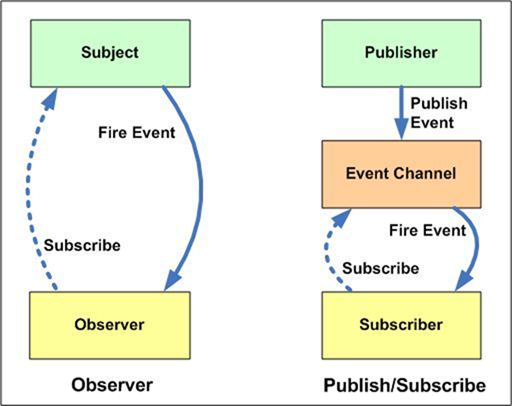
\includegraphics[width=0.6\textwidth]{images/Fig08.png}
    \caption{Отличие Subject -- Observer от Publisher -- Subscriber \cite{IMG_observer_vs_pub_sub}}
    \label{fig:Observer_vs_pub_sub}
\end{figure}


\subsubsection{Типы сообщений}

\paragraph{Configuration Message (адресованное)}
\begin{itemize}
  \item \texttt{Install}: 
  \[ (\mathit{id}_{\mathrm{recv}} :  \textit{\textbf{install}} : \mathit{id}_{\mathrm{sender}} : \textit{topic} : \textit{command}) \]
  Добавляет в локальный набор правил запись \((\mathit{id}_{\mathrm{sender}},\,\textit{topic}\to\textit{command})\).

  \item \texttt{Delete}: 
  \[ (\mathit{id}_{\mathrm{recv}} : \textit{\textbf{delete}} : \mathit{id}_{\mathrm{sender}} : \textit{topic} : \textit{command}) \]
  Удаляет из локального набора правил соответствующую запись.

  \item \texttt{Edit}: реализуется как последовательность \texttt{delete} старой и \texttt{install} новой записи.
\end{itemize}

\paragraph{Event Message (широковещательное)}
\[
(* : \textit{\textbf{event}} : \mathit{id}_{\mathrm{sender}} : \textit{topic} : \textit{payload})
\]


\subsubsection{Алгоритм обработки Event Message}

\begin{enumerate}
  \item \textbf{Приём и валидация.} Проверка контрольной суммы и механизма аутентификации; в случае неуспеха сообщение отбрасывается.
  \item \textbf{Фильтрация.} По полям $(\mathit{id}_{\mathrm{sender}},\,\textit{topic})$ отбираются все правила из локального набора.
  \item \textbf{Выполнение кода.} Для каждого найденного правила последовательно выполняются:
    \begin{enumerate}
      \item \textit{payload} из Event Message;
      \item \textit{command} из правила.
    \end{enumerate}
\end{enumerate}

\subsubsection{Формат команд и правила (Rules)}
Каждое устройство хранит набор правил:
\[
\textit{Rule} \equiv (\mathit{id}_{\mathrm{sender}},\,\textit{topic},\,\textit{command}),
\]

Оба фрагмента — \textit{payload} и \textit{command} — могут быть произвольными JS-конструкциями, например:

\paragraph{Пример простого payload и command}
\begin{verbatim}
// payload
Switcher02 = 1;

// command
LedSwitch(Switcher02);
\end{verbatim}

\paragraph{Пример с условием}
\begin{verbatim}
// payload
temp = 17.3;

// command
if (temp < 18) {
  PowerSwitch(1);
} else{
  PowerSwitch(0);
}
\end{verbatim}




%%%%%%%%%%%%%%%%%%%%%%%%%%%%%%%%%%%%%%%%%%%%%%%%%%%%%%%%%%%%%%%%%%%%%%%%%%%%%%%%%%%%%%%%%%%%%%%%%%%%%%%%%%%%%%%%%%%%%%%%%%%%%%%%%%%%%%%%%%%%%%%%%%%%%%%%%%%%%%%%%%%%%%%%%%%%%
%%%%%%%%%%%%%%%%%%%%%%%%%%%%%%%%%%%%%%%%%%%%%%%%%%%%%%%%%%%%%%%%%%%%%%%%%%%%%%%%%%%%%%%%%%%%%%%%%%%%%%%%%%%%%%%%%%%%%%%%%%%%%%%%%%%%%%%%%%%%%%%%%%%%%%%%%%%%%%%%%%%%%%%%%%%%%
%%%%%%%%%%%%%%%%%%%%%%%%%%%%%%%%%%%%%%%%%%%%%%%%%%%%%%%%%%%%%%%%%%%%%%%%%%%%%%%%%%%%%%%%%%%%%%%%%%%%%%%%%%%%%%%%%%%%%%%%%%%%%%%%%%%%%%%%%%%%%%%%%%%%%%%%%%%%%%%%%%%%%%%%%%%%%
%                                                                                                                                                                           %
%                                                             ГЛАВА IV. Распределённый отказаустойчивый кластер.                                                            %
%                                                                                                                                                                           %
%%%%%%%%%%%%%%%%%%%%%%%%%%%%%%%%%%%%%%%%%%%%%%%%%%%%%%%%%%%%%%%%%%%%%%%%%%%%%%%%%%%%%%%%%%%%%%%%%%%%%%%%%%%%%%%%%%%%%%%%%%%%%%%%%%%%%%%%%%%%%%%%%%%%%%%%%%%%%%%%%%%%%%%%%%%%%
%%%%%%%%%%%%%%%%%%%%%%%%%%%%%%%%%%%%%%%%%%%%%%%%%%%%%%%%%%%%%%%%%%%%%%%%%%%%%%%%%%%%%%%%%%%%%%%%%%%%%%%%%%%%%%%%%%%%%%%%%%%%%%%%%%%%%%%%%%%%%%%%%%%%%%%%%%%%%%%%%%%%%%%%%%%%%
%%%%%%%%%%%%%%%%%%%%%%%%%%%%%%%%%%%%%%%%%%%%%%%%%%%%%%%%%%%%%%%%%%%%%%%%%%%%%%%%%%%%%%%%%%%%%%%%%%%%%%%%%%%%%%%%%%%%%%%%%%%%%%%%%%%%%%%%%%%%%%%%%%%%%%%%%%%%%%%%%%%%%%%%%%%%%
\newpage

\section{Глава 4. Распределённый отказаустойчивый кластер.}


\begin{figure}[h]
    \centering
    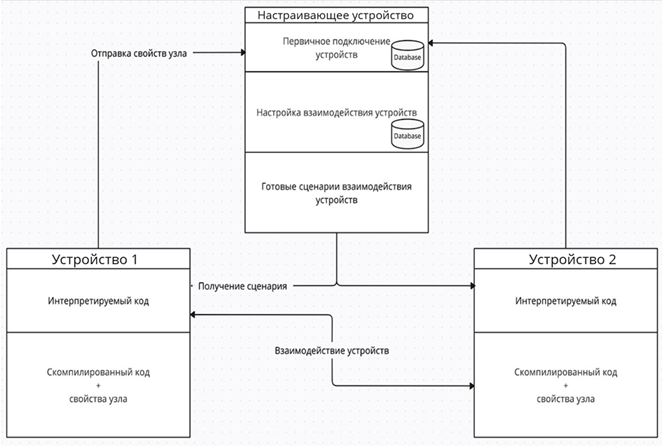
\includegraphics[width=0.8\textwidth]{images/Fig09.png}
    \caption{Пример взаимодействий конечных устройств}
    \label{fig:Connect_end_device_example}
\end{figure}


\begin{figure}[H]
    \centering
    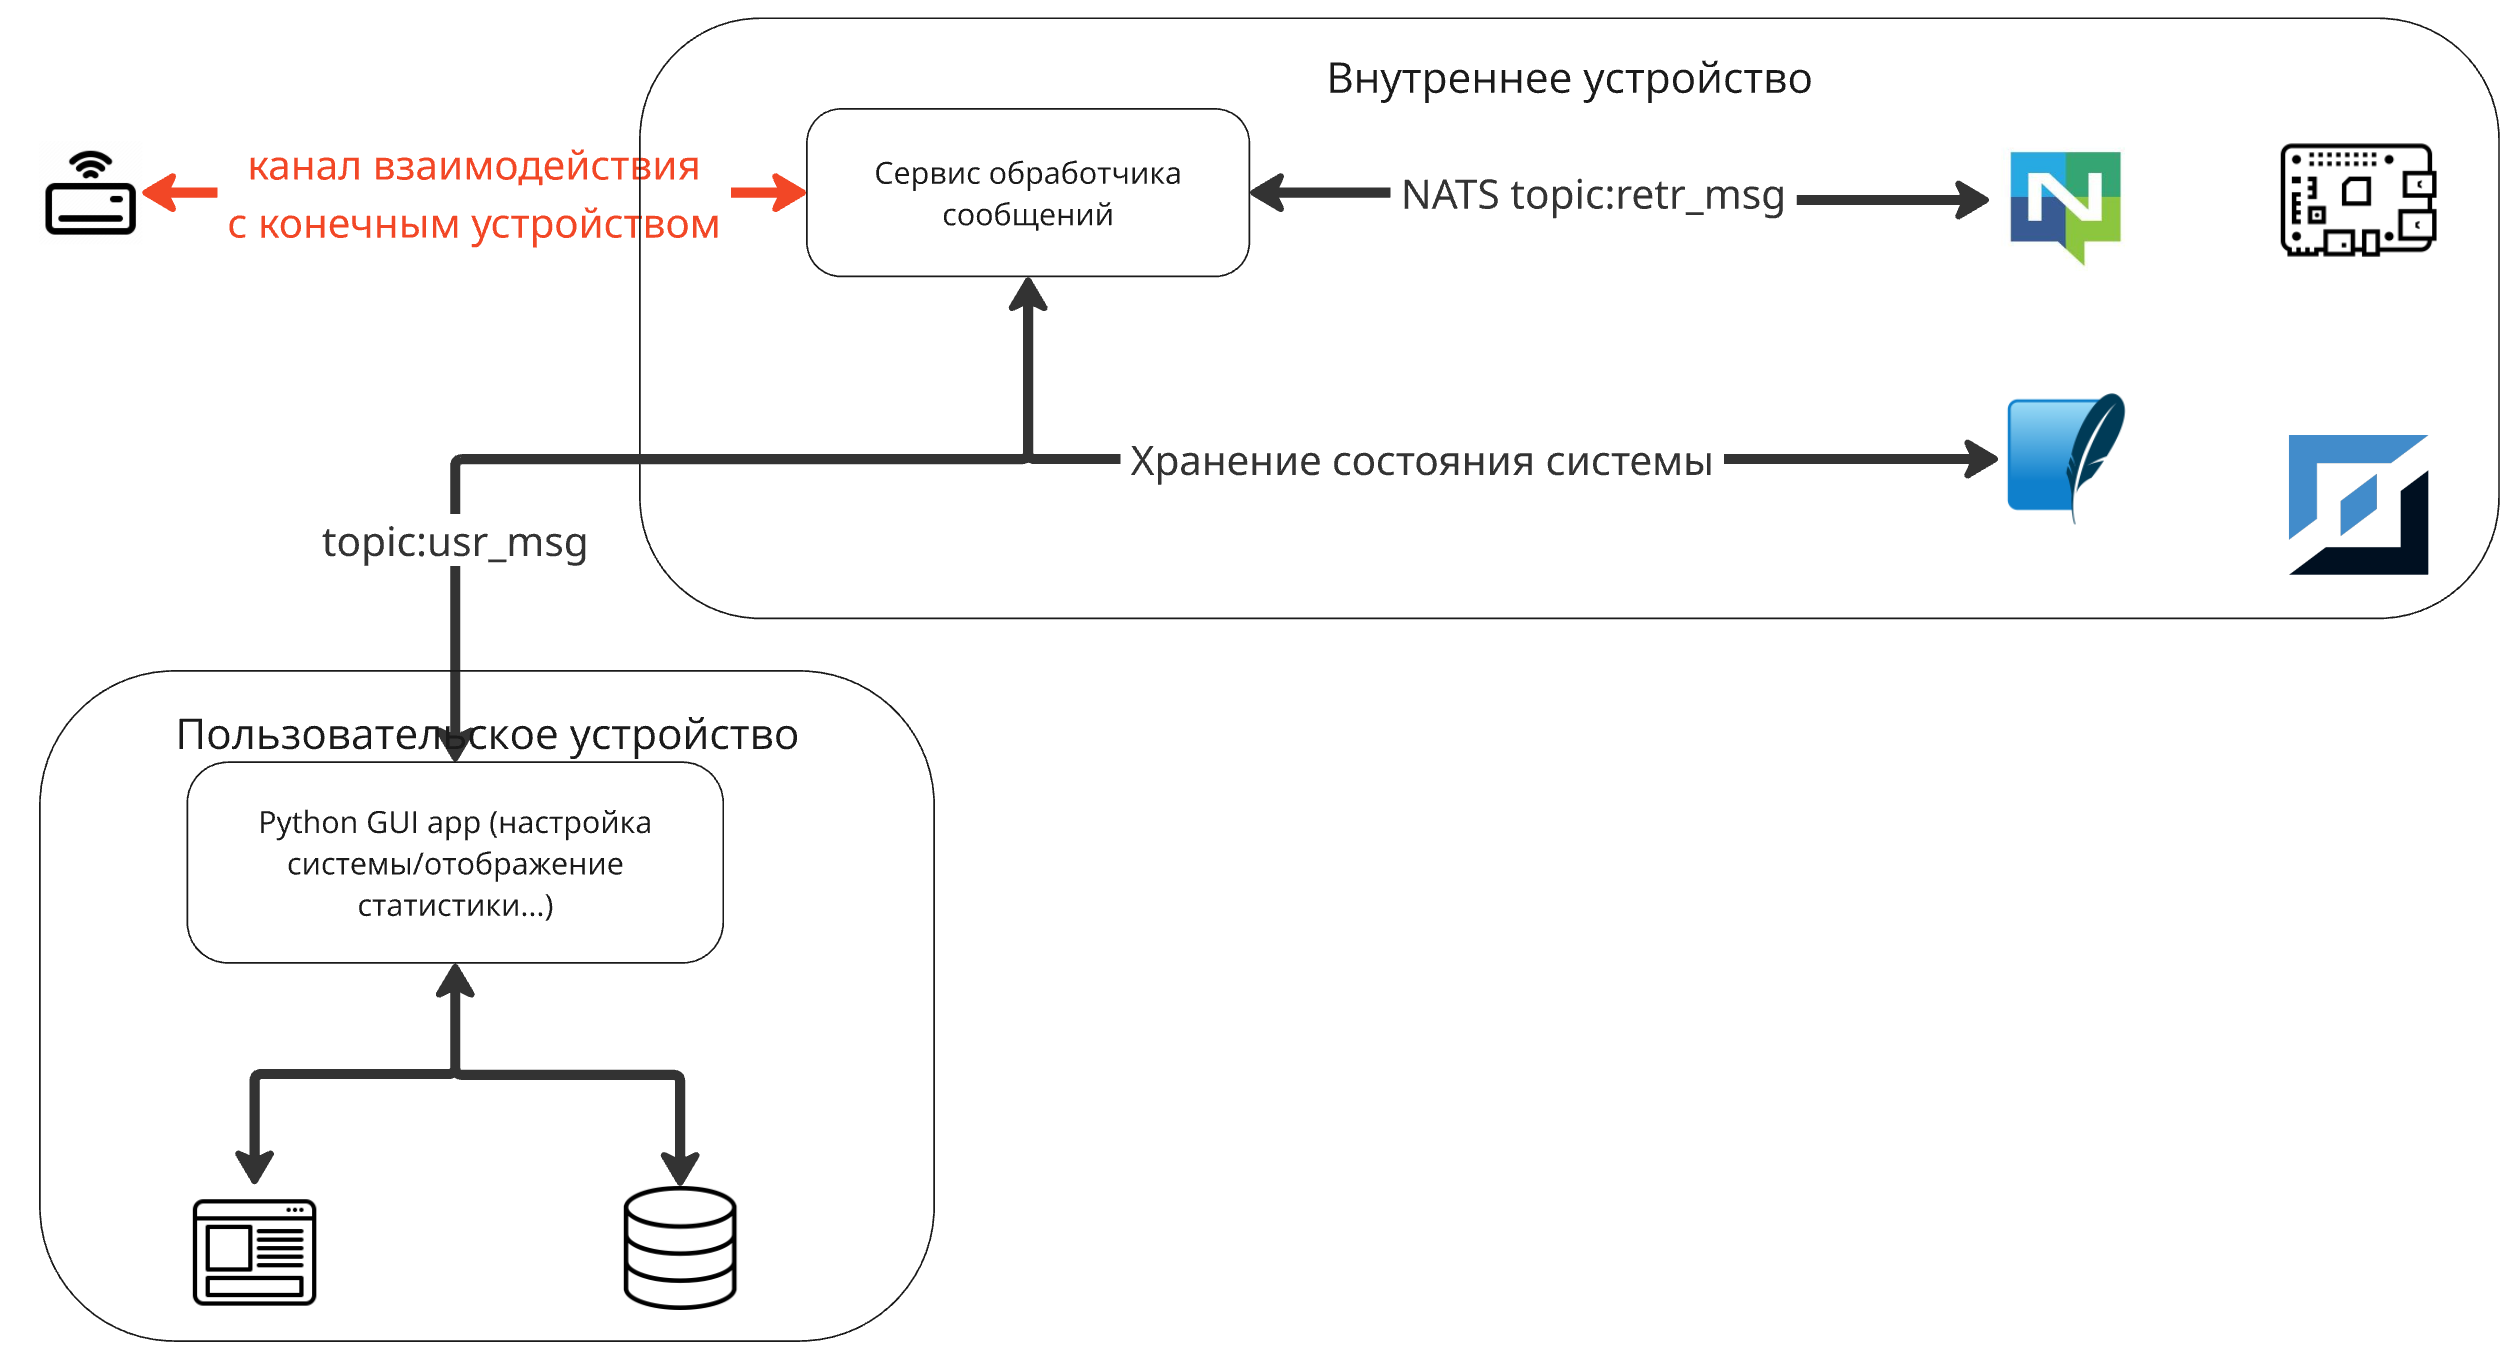
\includegraphics[width=0.8\textwidth]{images/InternalSystemDesign.png}
    \captionsetup{justification=centering}
    \caption{Компонентная структура и процессы взаимодействия в\\кластере K0s предложеннной системы}
    \label{fig:InternalSystemDesign}
\end{figure}


Шлюзы-ретрансляторы -- кластер K0s -- при выходе из строя какого-то узла, например, зоны
K, перестанут обрабатываться межзонные события, связанные с зоной К. При этом функционал внутри и вне зоны
К не изменится.



\subsection{Добавление устройств и настройка сценариев}

Система домашней автоматизации состоит из конечных устройств, связанных по радиоканалу, и шлюзов-ретрансляторов, представляющих собой одноплатные компьютеры с установленными сервисами \texttt{k0s}. Настройка системы выполняется через единое графическое приложение, содержащее кнопку для начала настройки, поле для изменения параметров и кнопку для применения изменений.

\begin{enumerate}[label=\textbf{\arabic*.}]
    \item \textbf{Перевод системы в режим настройки.} 
    
    Пользователь нажимает кнопку <<Начать настройку системы>> в графическом интерфейсе. Приложение отправляет управляющую команду на все шлюзы-ретрансляторы, которые, в свою очередь, передают её конечным устройствам. Устройства переходят из режима эксплуатации в режим настройки и готовы к приёму новой конфигурации.
    
    \item \textbf{Внесение и отправка изменений.} 
    
    Через предоставленное текстовое или графическое поле в приложении вносятся необходимые изменения конфигурации. Это могут быть новые сценарии взаимодействия, логика работы исполнительных устройств и параметры ретрансляции сообщений. После завершения редактирования пользователь нажимает кнопку <<Применить настройки>>, и новая конфигурация передаётся на шлюзы-ретрансляторы.
    
    \item \textbf{Распространение конфигурации на конечные устройства.} 
    
    Шлюзы-ретрансляторы получают обновлённую конфигурацию и передают её по радиоканалу на исполнительные устройства. Датчики не требуют настройки, так как они только передают сообщения. Исполнительные устройства анализируют входящие сигналы и запускают соответствующие действия по заданным сценариям. После успешного применения настроек система может быть переведена обратно в режим работы тем же интерфейсом.
\end{enumerate}






\newpage

\section{Глава 3}

\subsection{Графический интерфейс}
Был написано графическое приложение рис.~\ref{fig:GUI_base} на языке Python c использованием фреймворка Qt, в котором производилась настройка системы и ее отладка.

\begin{figure}[H]
    \centering
    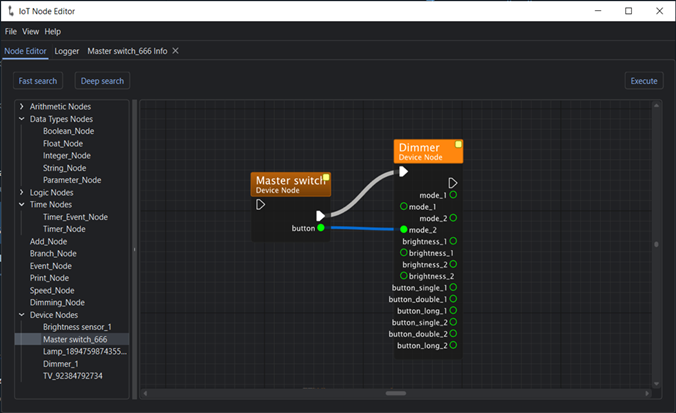
\includegraphics[width=0.8\textwidth]{images/Fig11.png}
    \captionsetup{justification=centering}
    \caption{Графическое приложение с созданным внутри\\сценарием для конечных устройств}
    \label{fig:GUI_base}
\end{figure}

Графический интерфейс позволяет прописывать и более сложные сценарии взадимодействия устройств, что можно увидеть на рис.~\ref{fig:GUI_adv}

\begin{figure}[H]
    \centering
    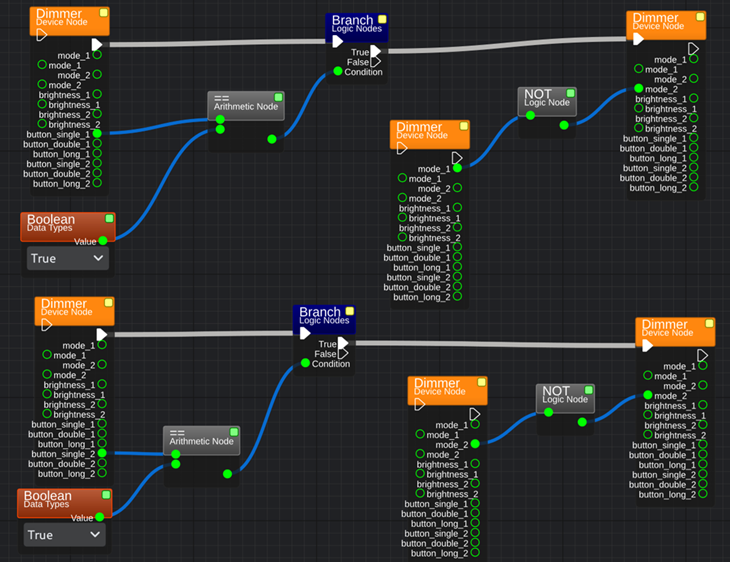
\includegraphics[width=0.8\textwidth]{images/Fig12.png}
    \caption{Пример более сложного сценария взаимодействия устройств}
    \label{fig:GUI_adv}
\end{figure}

\subsection{Планировщик}
Было опробовано два варианта распределения сценариев: их хранение и исполнение на устройстве-отправителе, порождающем событие и хранение сценариев на устройстве-исполнителе. В рамках проведенных экспериментов было установлено, что некоторые сложные команды, последовательный набор действий для первого варианта проводят к значительному увеличению времени обработки и излишней загруженности радиоканала, что потенциально уменьшает максимальное число устройств в системе.
Планировщик осуществляет преобразование визуальных узлов и связей в JS код, выполняя синтаксический анализ, преобразованием узлов в лексемы с последующем объединением их в единый исполняемый файл. Так же в задачи планировщика входит разбиение файла настроек на компоненты связанности и определение целевого устройства, на которое будет отправлен сценарий.
Также для дальнейшего тестирования система была сконфигурирована для работы с использованием ЦУД и для распределенной работы.

\newpage

\section{Глава 4}
\subsection{Тестирование и полученные оценки}
Для корректности тестирования и сравнимости подходов, ввиду отличия протоколов передачи данных, использования разных
микроконтроллеров в существующих системах и иных отличий, исходная система была переконфигурирована для работы как с
ЦУД, так и без ЦУД. Таким образом, проведя замеры задержек от возникновения события до реакции, можно оценить численно
преимущество предложенной архитектуры. В таблице приведены результаты замеров на каждом этапе: время передачи
пакета сообщения, время обработки события для каждой системы, что позволило использовать эти данные без привязки к
конкретной реализации. Были проведены замеры времени задержек выполнения программы на микроконтроллере STM32F411
(25МГц), выступавшим в качестве конечного устройства, и одноплатным компьютером Raspberry pi 3b+. Тестирование
одноплатного компьютера проводилось на системе Raspberry Pi OS 19.11, базирующейся на Debian 12. Использовался GCC 15
с опциями: <<-mcpu=native, -O2>>. При тестировании микроконтроллеров использовалась STM32duino FreeRTOS v10.3.2 с
библиотекой RadioLib v7.1.2. Радиомодули, представленные SI4432, использовались со стандартными параметрами.

\begin{table}[h!]
    \centering
    \begin{tabular}{|>{\centering\arraybackslash}p{1cm}|>{\centering\arraybackslash}p{8cm}|>{\centering\arraybackslash}p{2.5cm}|}
    \hline
    \textbf{п/п} & \textbf{Тип операции} & \textbf{Время операции} \\
    \hline
    1 & Передача в рамках одной зоны & 197 мс \\
    \hline
    2 & Выполнение 1 примитива интерпретатора на микроконтроллере & 18 мс \\
    \hline
    3 & Выполнение 1 примитива интерпретатора на одноплатном компьютере & 0{,}24 мс \\
    \hline
    4 & Общая задержка системы при использовании ЦУД & 407 мс \\
    \hline
    5 & Общая задержка системы без использования ЦУД & 231 мс \\
    \hline
    6 & Задержка СУД <<Умный дом с Алисой>> от Яндекс & $\sim$470 мс \\
    \hline
    \end{tabular}
    \caption{Среднее время выполнения операций}
\end{table}
    


Использовалось готовое решение на базе протокола Zigbee с ЦУД в виде YNDX-00510 \cite{YNDX_hub} и
лампой YNDX-00558. Лучшим способом сокращения задержек в СУД является уменьшение задержек в передаче
информации.Предложенный выше подход позволяет почти в вдвое сократить задержку (в рамках тестирования спроектированной
СУД) и более чем втрое по сравнению с представленными на рынке решениями.

\subsection{Вывод}
Предложен подход к построению распределенной системы домашней автоматизации, проведено сравнение с решением,
представленным на рынке. В дальнейшем предполагается исследовать возможные
уязвимости данной системы, построить и протестировать прототип распределенной системы с использованием шлюзов-ретрансляторов,
объединенных в единую сеть посретсвом VPN.

\newpage
\begin{thebibliography}{40}
\bibitem{wirelessNetProtocols} Колыбельников~А.\:И. Обзор технологий беспроводных сетей // ТРУДЫ МФТИ. 2012. Т.~4. №~2 С.~3--29.
\bibitem{Rus_alternative} Шерчков~А.\:В. Анализ существующих технических решений <<Умный дом>> // Молодежный вестник Уфимского государственного авиационного технического университета. 2020. №~1 С.~153--155.
\bibitem{WifiSmartHome} Montori~F., Contigiani~R., Bedogni~L., Is WiFi suitable for energy efficient IoT deployments? A performance study // 2017 IEEE 3rd International Forum on Research and Technologies for Society and Industry (RTSI). 2017. pp. 1-5, doi: 10.1109/RTSI.2017.8065943.
\bibitem{smart_home_review} Тукмачева~Ю.\:А. Обзор и анализ автоматизированных систем <<Умный дом>>, представленных на российском сегменте рынка // Вестник науки. 2022. Т.~4. №~10 С.~139--144.
\bibitem{SecuritySmartHome} Некрасов~П.\:В., Жариков~А.\:М., Козин~Д.\:А. Обеспечение безопасности беспроводных каналов связи киберфизических систем типа «Умный дом» // Безопасность информационных технологий. 2024. Т.~31. №~1 С.~54--62.
\bibitem{SecuritySmartHome2} Vardakis~G., Hatzivasilis~G., Koutsaki~E., Papadakis~N. Review of smart-home security using the internet of things // Electronics. 2024. No~13 P.~33--43.
\bibitem{YNDX_hub} Центр умного дома «Яндекс Хаб» модель YNDX-00510. Инструкция по эксплуатации [Электронный ресурс]: \url{URL: https://yastatic.net/s3/doc-binary/src/support/smart-home/hub/hub-manual.pdf} (дата обращения: 17.03.2025).
\bibitem{BLE_mesh_spec} Specifications and Documents Mesh Protocol [Электронный ресурс]: \url{URL: https://www.bluetooth.com/specifications/specs/html/?src=MshPRT_v1.1/out/en/index-en.html} (дата обращения: 11.05.2025).
%Zigbee & Zigbee Pro
\bibitem{ZIGBEE_SPEC_R23} Zigbee Specification Revision 23 [Электронный ресурс]: \url{https://csa-iot.org/wp-content/uploads/2023/04/05-3474-23-csg-zigbee-specification-compressed.pdf} (дата обращения: 20.05.2025).

\bibitem{IEEE802_15_4_2020} IEEE Std 802.15.4-2020: IEEE Standard for Low-Rate Wireless Personal Area Networks (LR-WPANs) [Электронный ресурс]: \url{URL: https://standards.ieee.org/standard/802_15_4-2020.html} (дата обращения: 20.05.2025).

\bibitem{Fault_Tolerance_ZigBee} Richard Alena, Ray Gilstrap, Jarren Baldwin, Thom Stone, Pete Wilson. Fault Tolerance in ZigBee Wireless Sensor Networks // NASA Ames Research Center, Moffett Field [Электронный ресурс]: \url{URL: https://ntrs.nasa.gov/api/citations/20110012426/downloads/20110012426.pdf?utm_source=chatgpt.com} (дата обращения: 20.05.2025).

%\bibitem{ZigBee_test} Ferrari, Gianluigi & Medagliani, Paolo & Piazza, S. & Martalo, Marco. Wireless Sensor Networks: Performance Analysis in Indoor Scenarios. EURASIP Journal on Wireless Communications and Networking. 2007.

%\bibitem{ZCL_SPEC} ZigBee Cluster Library Specification (07-5123-08), Connectivity Standards Alliance [Электронный ресурс]: \url{https://zigbeealliance.org/wp-content/uploads/2021/10/07-5123-08-Zigbee-Cluster-Library.pdf} (дата обращения: 20.05.2025).

\bibitem{NXP_JNUG3101} Zigbee Pro Stack User Guide (JN-UG-3101), NXP Semiconductors [Электронный ресурс]: \url{URL: https://www.nxp.com/docs/en/user-guide/JN-UG-3101.pdf} (дата обращения: 20.05.2025).

\bibitem{CSMA_article} Simon S. Lam, A Carrier Sense Multiple Access Protocol for Local Networks // Computer Networks. 1976. Vol.~4 Issue~1 P.~21--32,

\bibitem{IMG_RTOS_architectures} Qutqut M., Al-Sakran A., Almasalha F., Hassanein H. // Comprehensive Survey of the IoT Open Source OSs. IET Wireless Sensor Systems. 2018.

%images
\bibitem{IMG_protocol_compare} Сравнительный анализ стандартов связи для сетей IoT [Электронный ресурс]: \url{URL: https://habr.com/ru/companies/msw/articles/720518/} (дата обращения: 11.05.2025).

\bibitem{IMG_protocol_compare_power_eff} Wi-Fi HaLow™ and LoRaWAN: How do the technologies compare? [Электронный ресурс]: \url{URL: https://dev.wi-fi.org/zh-hans/beacon/y-zachary-freeman/wi-fi-halow-and-lorawan-how-do-the-technologies-compare} (дата обращения: 11.05.2025).

\bibitem{IMG_observer_vs_pub_sub} Observer vs Pub-Sub [Электронный ресурс]: \url{URL: https://habr.com/ru/articles/270339/} (дата обращения: 11.05.2025).

\bibitem{IMG_BLE_topologies} Generic Access Profile (GAP) Roles [Электронный ресурс]: \url{URL: https://developerhelp.microchip.com/xwiki/bin/view/applications/ble/introduction/bluetooth-architecture/bluetooth-host-layer/gap/roles/} (дата обращения: 19.05.2025).

\bibitem{IMG_Zigbee_profile} Bachelor Seminar Paper  [Электронный ресурс]: \url{URL: https://www.auto.tuwien.ac.at/bib/pdf_TR/TR0148.pdf} (дата обращения: 20.05.2025).

\end{thebibliography}

\newpage
\appendix
\renewcommand{\thesection}{\Alph{section}} % Нумерация буквами A, B, C…

% Заголовок первого приложения
\section*{Приложение A. Исходные коды и дополнительные материалы}
\addcontentsline{toc}{section}{Приложение A. Исходные коды и дополнительные материалы}

\begin{enumerate}[label=\arabic*.]
  \item Solovjev D. Distributed smart home cluster  [Электронный ресурс]: 
        \url{URL: https://github.com/Dmitrij-Solovjev/distributed-smart-home-cluster}
        (дата обращения: 11.05.2025). \\
        \emph{Примечание:} Кластер на базе K0s с сервисами для ретрансляции сообщений и общей настройки системы.
        
  \item Solovjev D. IoT Base Device [Электронный ресурс]: 
        \url{URL: https://github.com/Dmitrij-Solovjev/IoT-Base-Device} 
        (дата обращения: 11.05.2025). \\
        \emph{Примечание:} Прошивка для микроконтроллера на FreeRTOS, реализующая логику домашней автоматизации.
\end{enumerate}


\end{document}